\documentclass[12pt]{beamer}

\usetheme{metropolis}

\usepackage{appendixnumberbeamer}

\usepackage{pgfplots}
\usepackage{import}
\usepackage{booktabs}
\usepackage{ctable}
\usepackage{dcolumn}

\usepackage{xspace}
\usepackage{graphicx}
\usepackage{subfig}
\usepackage{adjustbox} 
\newcommand{\themename}{\textbf{\textsc{metropolis}}\xspace}

\title{Getting started with Zotero}
\date{\today}
\author{Aengus Bridgman}
\institute{CSDC Winter School}

\begin{document}

\maketitle

\section{Installation}

\begin{frame} \frametitle{Installing 1: Download} \begin{figure}[!h] \centering
	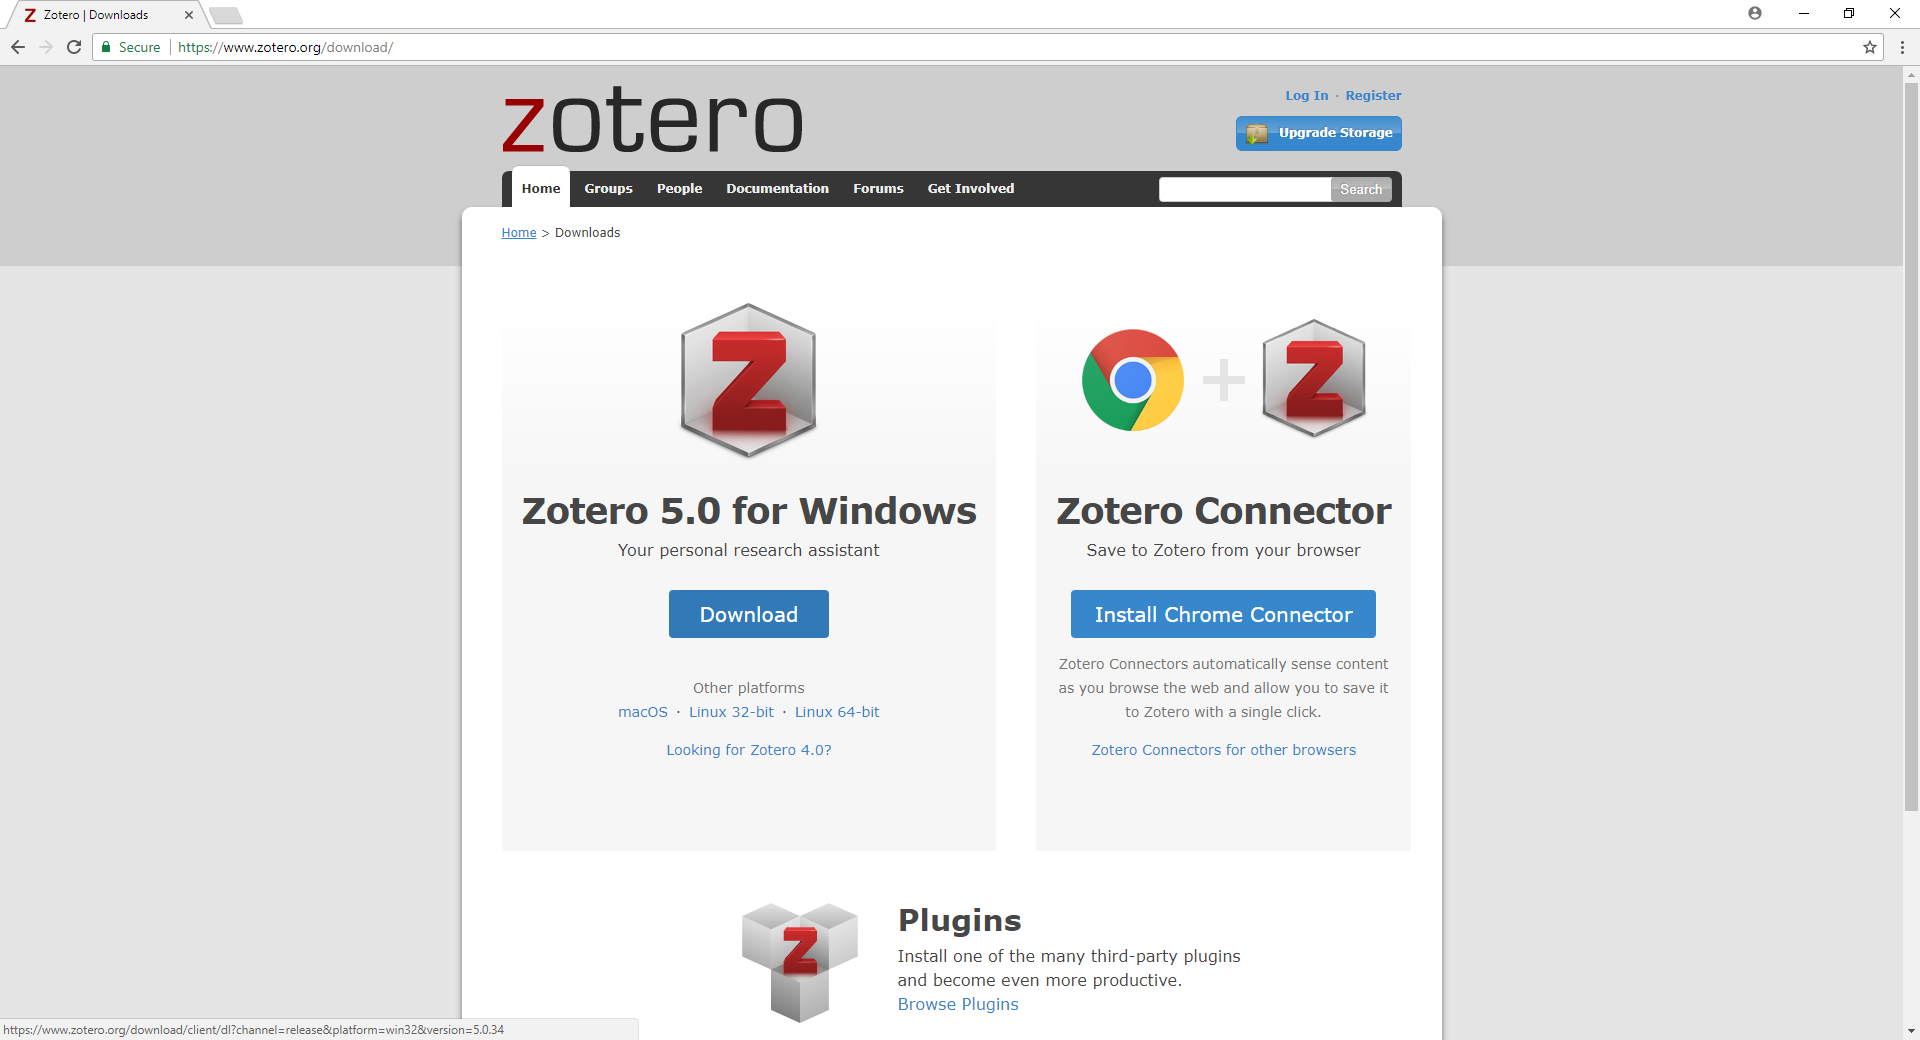
\includegraphics[height=3in, width = 4.25in,keepaspectratio]{zotero/install_1.png}
\end{figure} \end{frame}

\begin{frame} \frametitle{Installing 2: Setup type} \begin{figure}[!h] \centering
	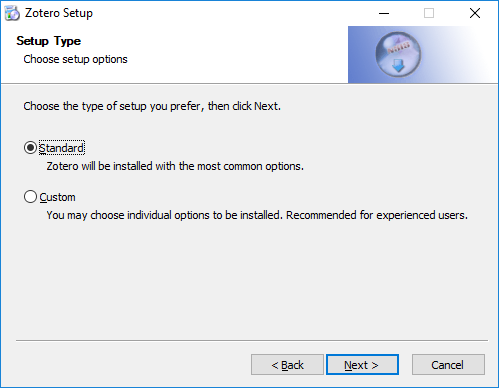
\includegraphics[height=3in, width = 4.25in,keepaspectratio]{zotero/install_2.png}
\end{figure} \end{frame}

\begin{frame} \frametitle{Installing 3: Patience} \begin{figure}[!h] \centering
	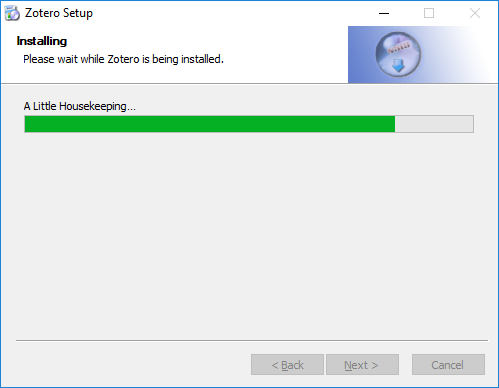
\includegraphics[height=3in, width = 4.25in,keepaspectratio]{zotero/install_3.png}
\end{figure} \end{frame}

\begin{frame} \frametitle{Installing 4: Connect if you wish...} \begin{figure}[!h] \centering
	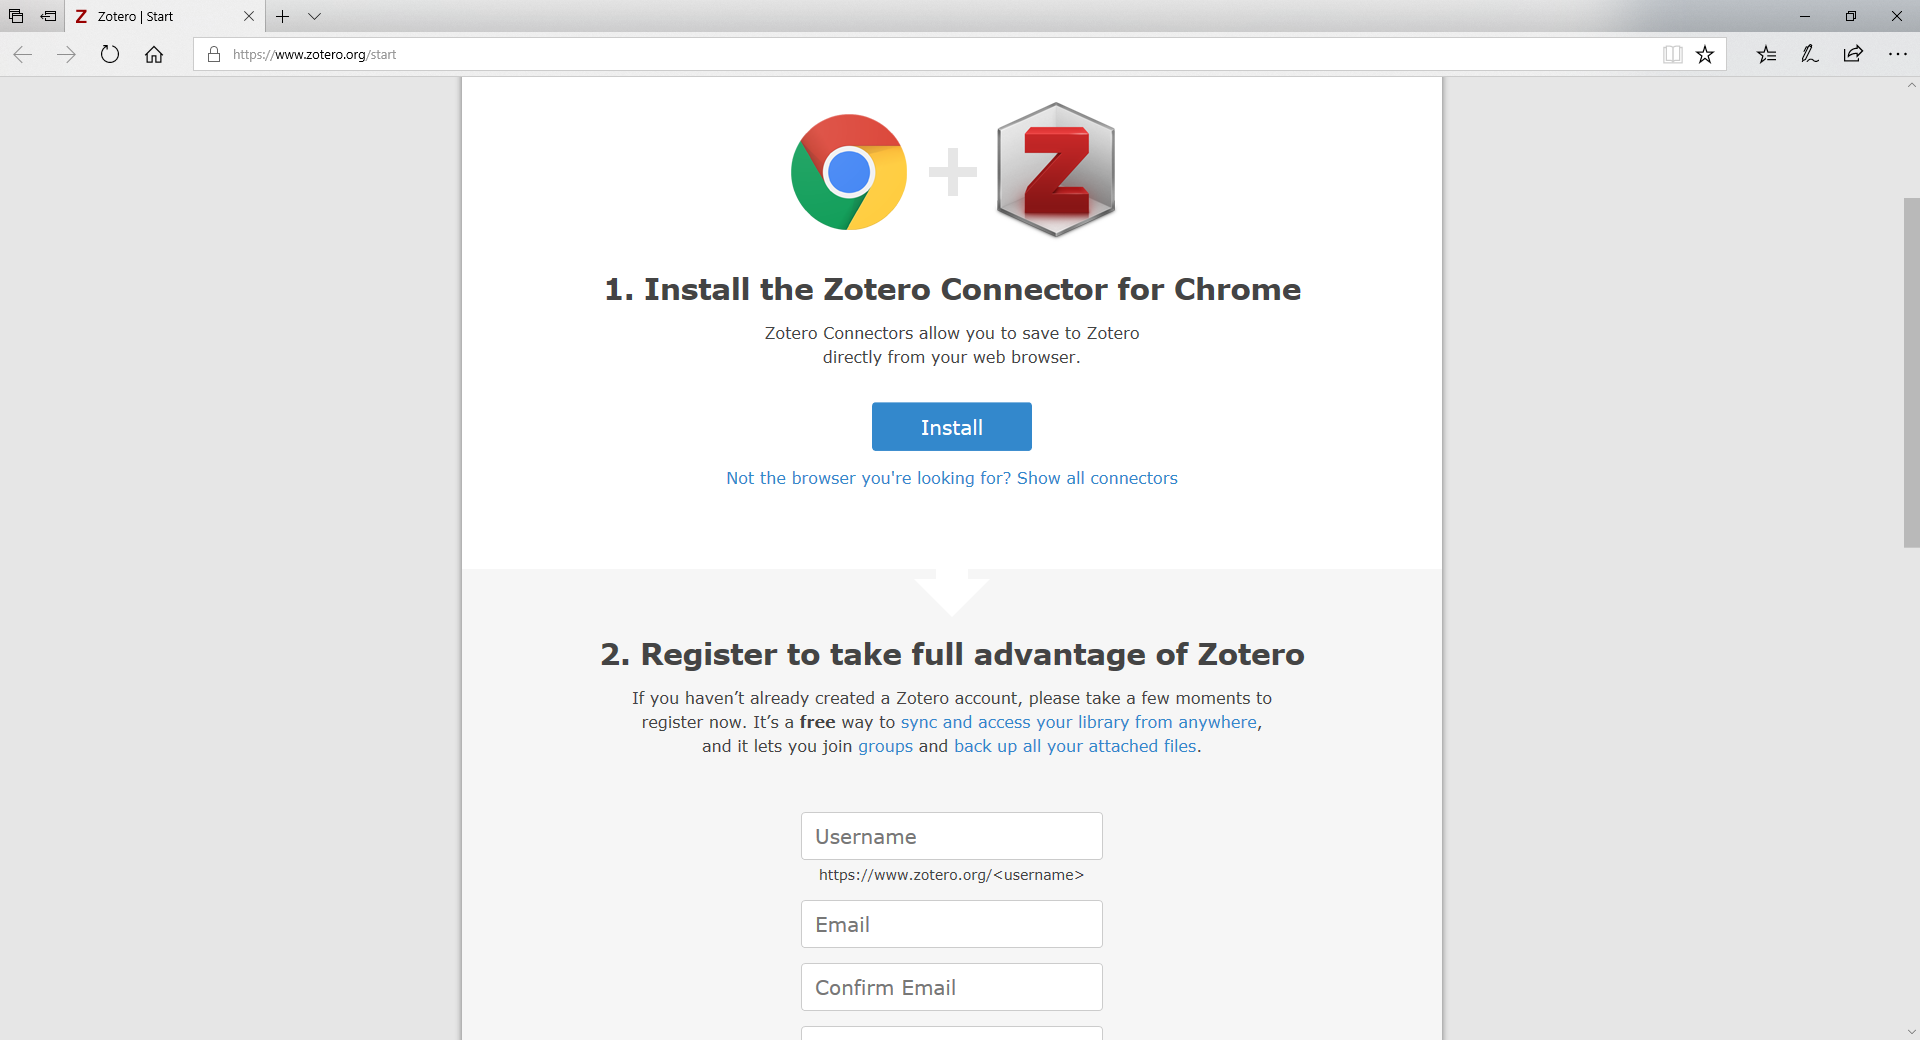
\includegraphics[height=3in, width = 4.25in,keepaspectratio]{zotero/install_4.png}
\end{figure} \end{frame}

\begin{frame} \frametitle{Installing 5: Welcome} \begin{figure}[!h] \centering
	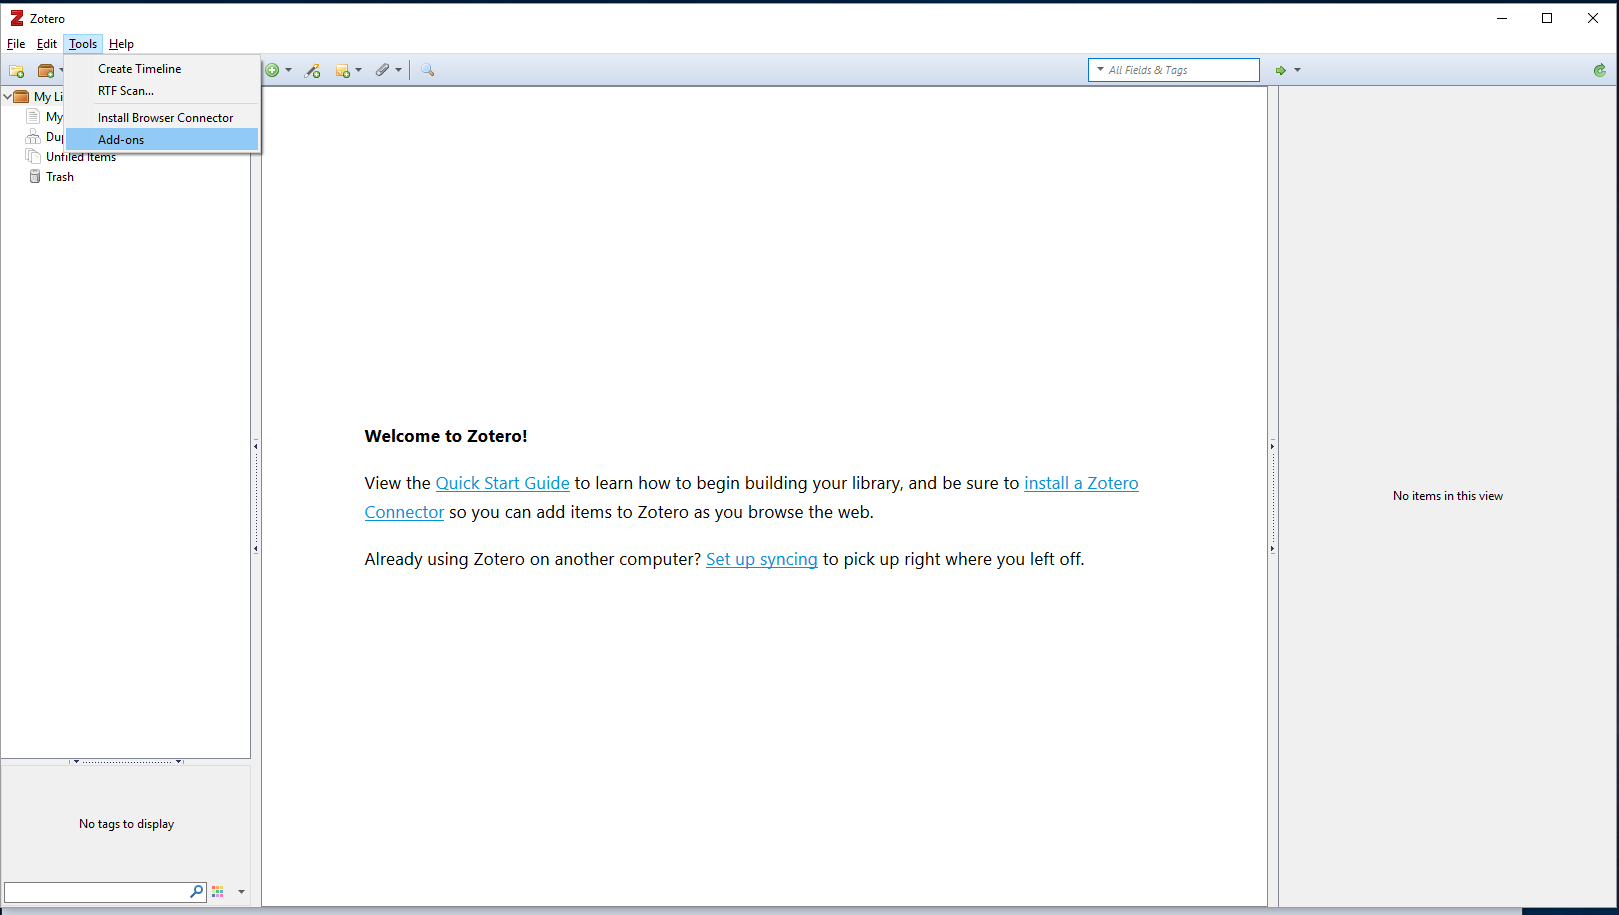
\includegraphics[height=3in, width = 4.25in,keepaspectratio]{zotero/install_5.png}
\end{figure} \end{frame}

\section{Installing Zotfile}

\begin{frame} \frametitle{ZotFile 1: Download} \begin{figure}[!h] \centering
	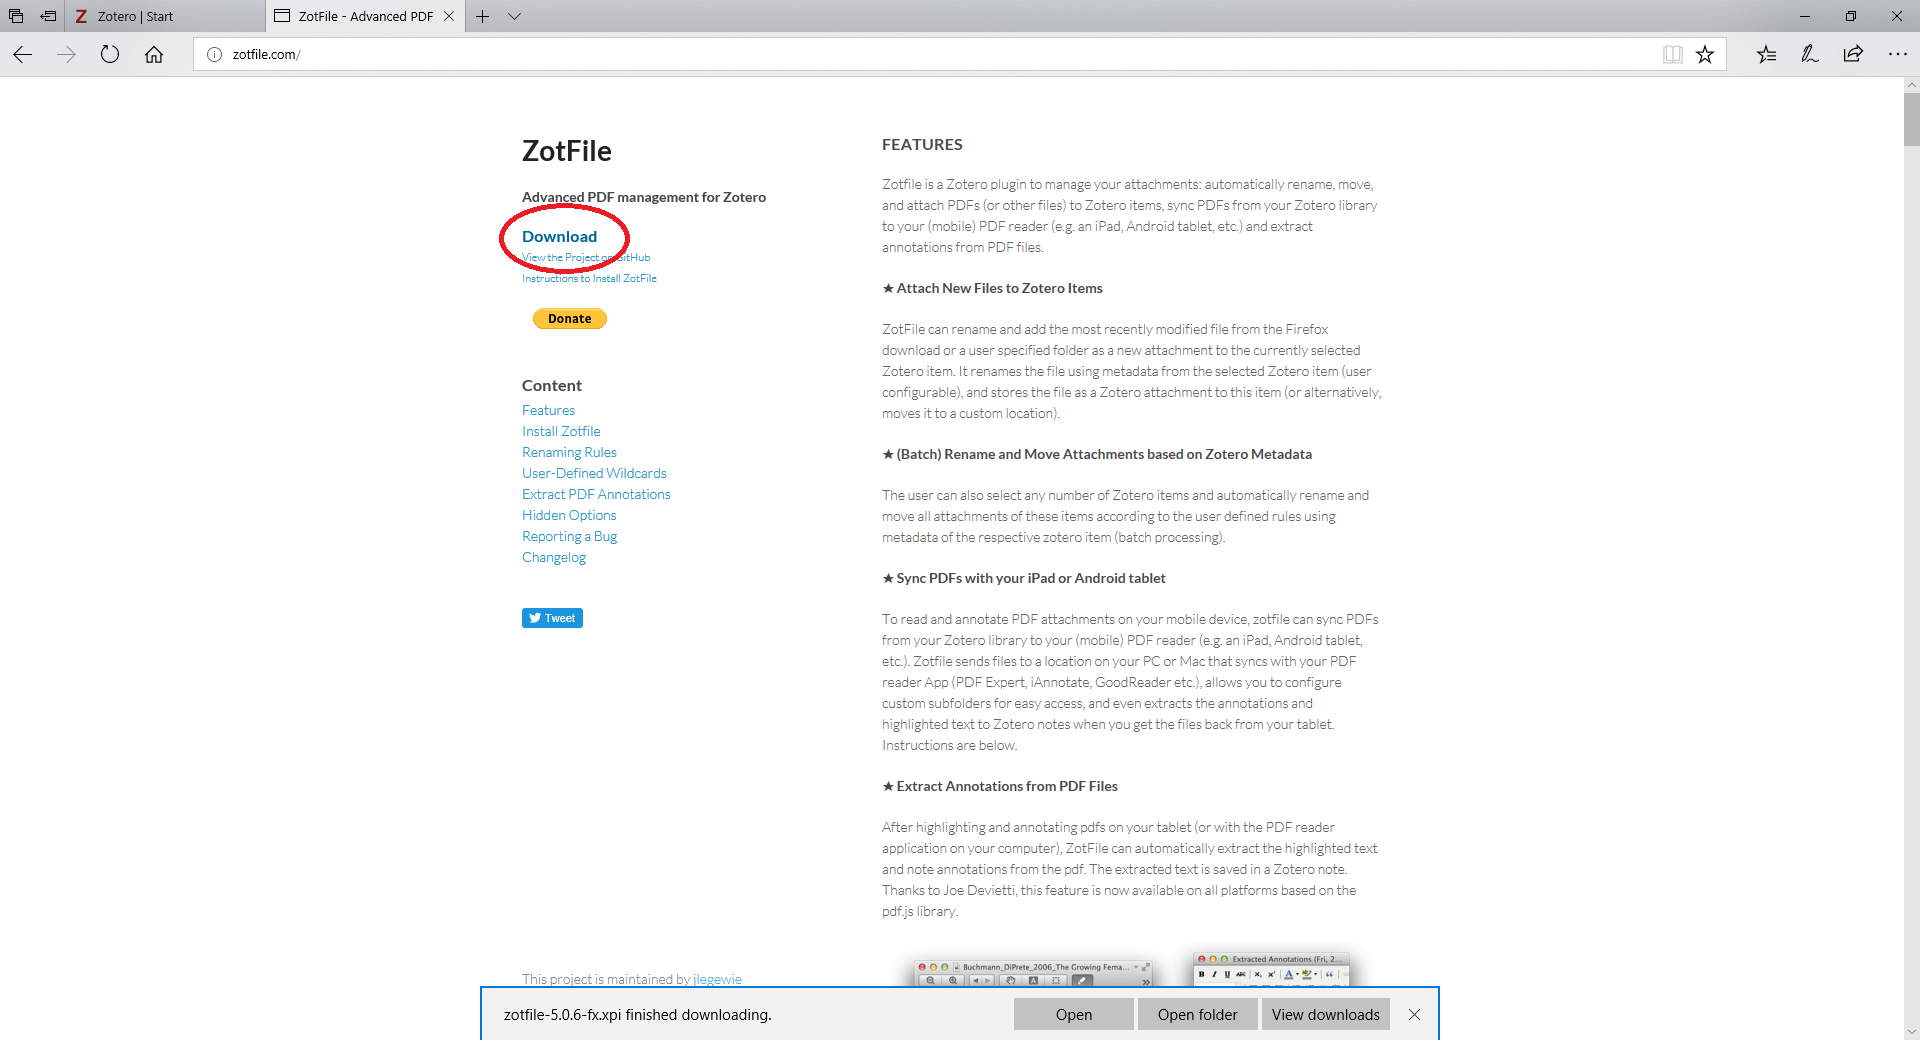
\includegraphics[height=3in, width = 4.25in,keepaspectratio]{zotero/zotfile_1.png}
\end{figure} \end{frame}

\begin{frame} \frametitle{ZotFile 2: Install add-ins for Zotero} \begin{figure}[!h] \centering
	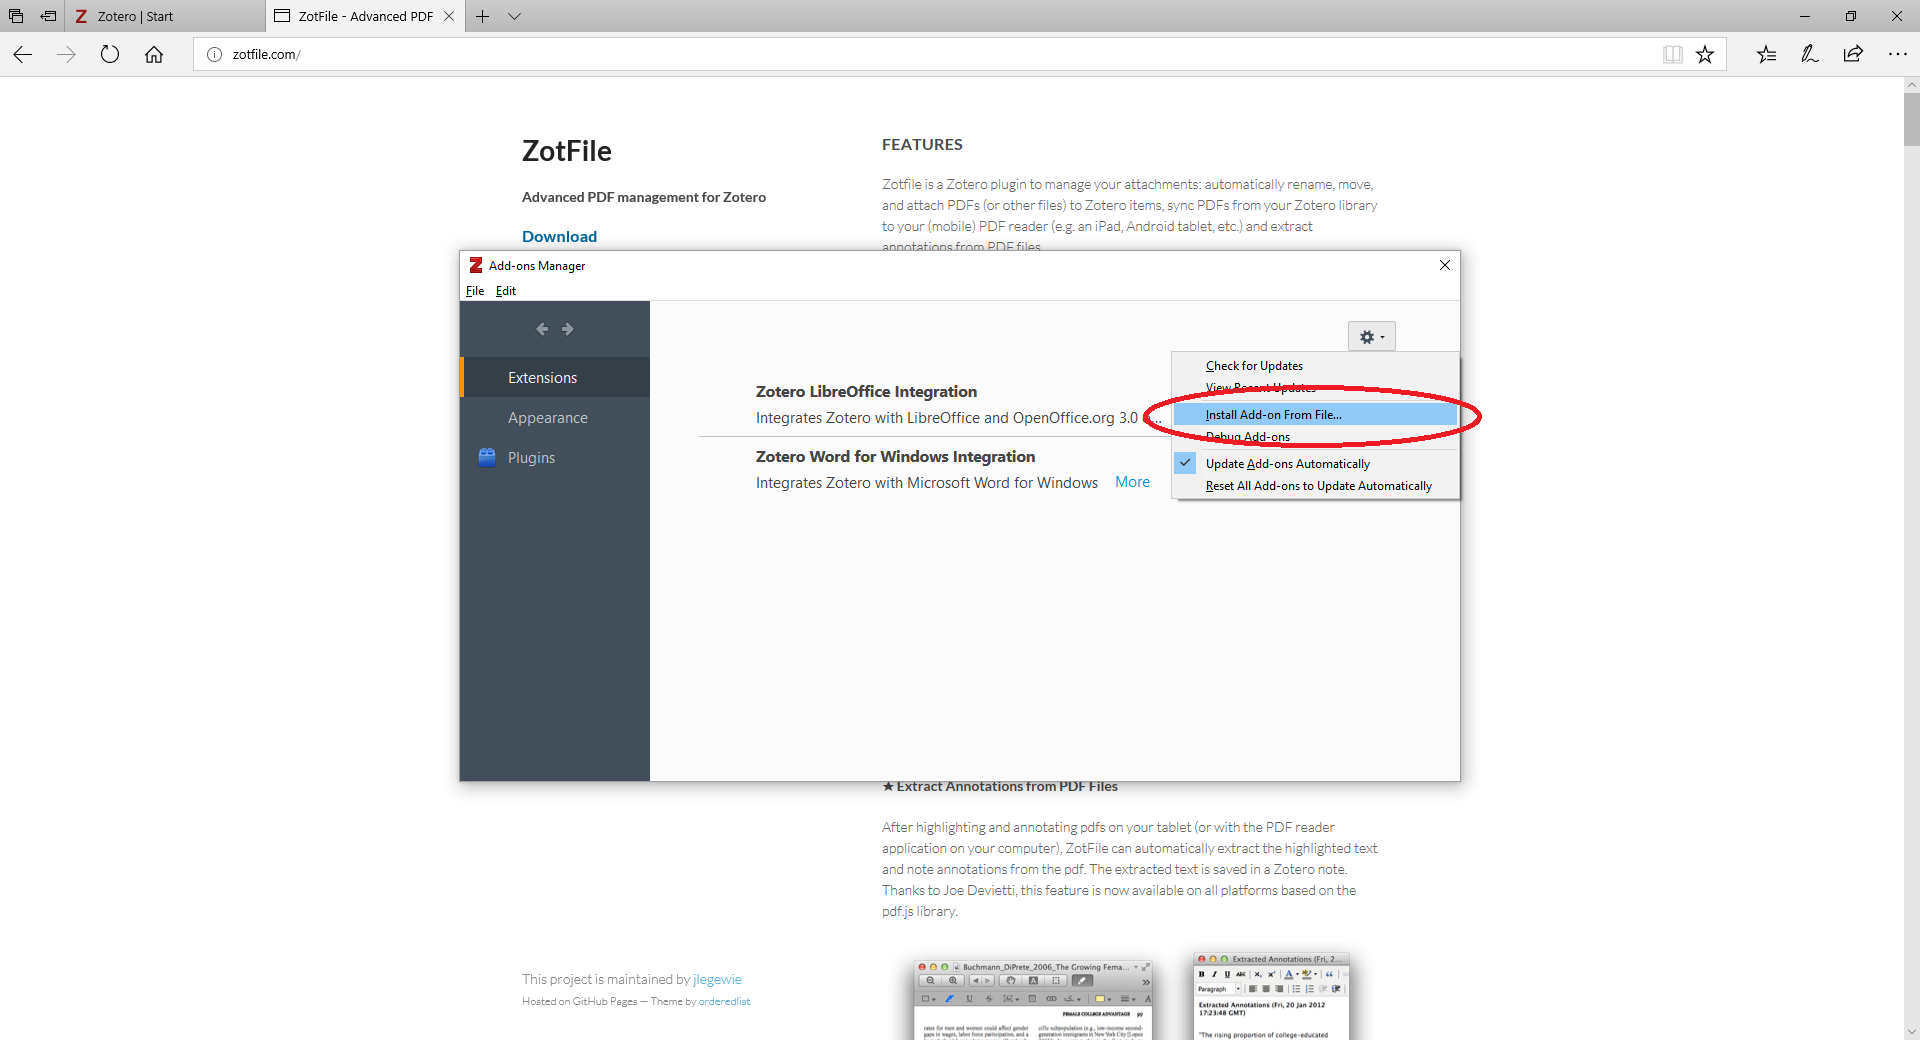
\includegraphics[height=3in, width = 4.25in,keepaspectratio]{zotero/zotfile_2.png}
\end{figure} \end{frame}

\begin{frame} \frametitle{ZotFile 3: Download} \begin{figure}[!h] \centering
	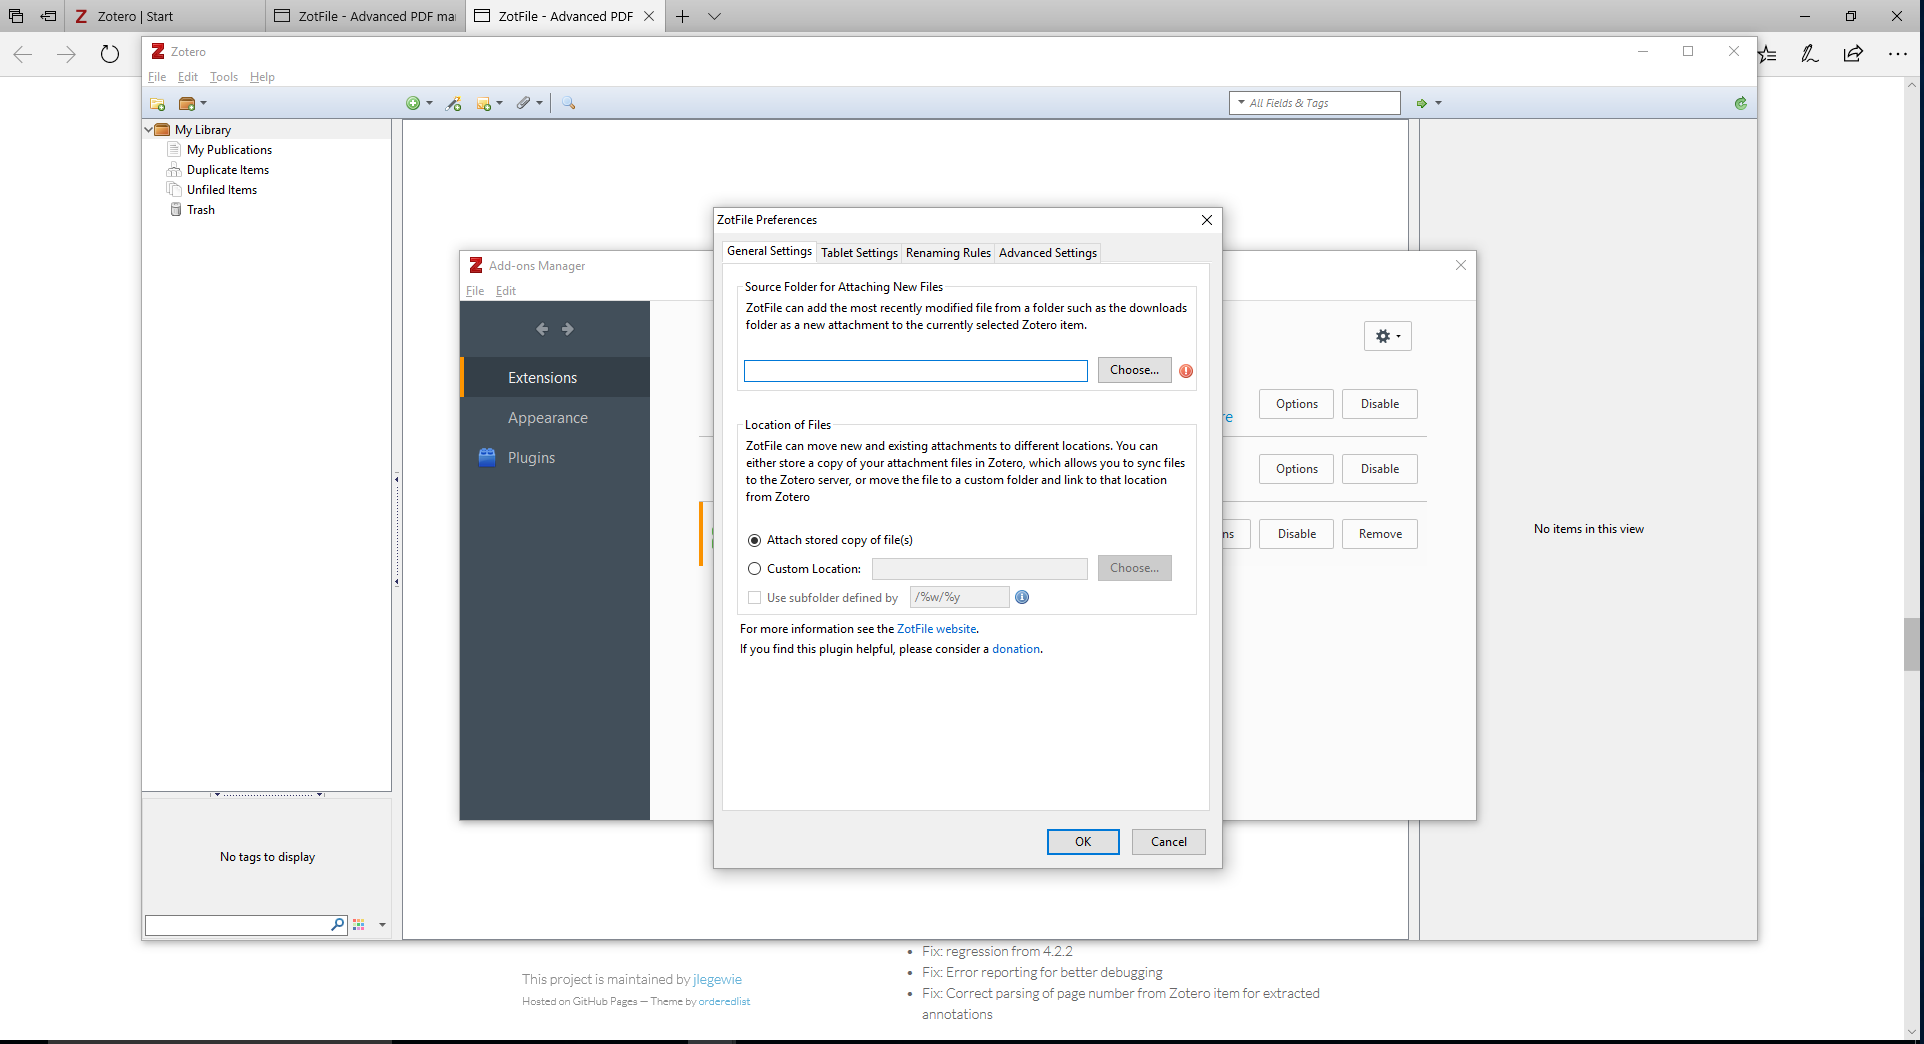
\includegraphics[height=3in, width = 4.25in,keepaspectratio]{zotero/zotfile_3.png}
\end{figure} \end{frame}

\begin{frame} \frametitle{ZotFile 4: Set up central document repository} \begin{figure}[!h] \centering
	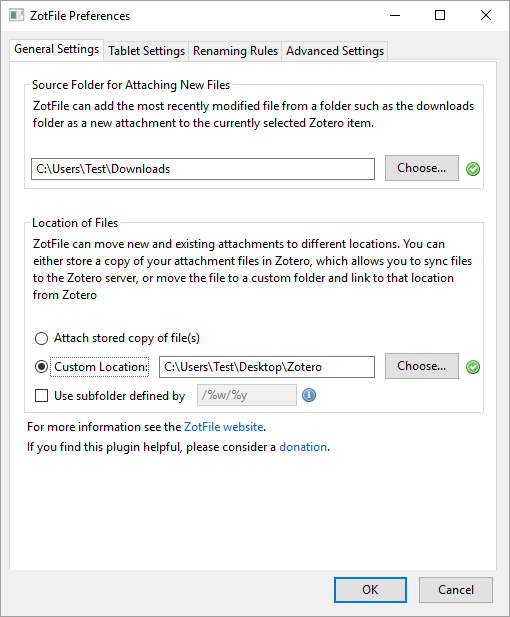
\includegraphics[height=3in, width = 4.25in,keepaspectratio]{zotero/zotfile_4.png}
\end{figure} \end{frame}

\begin{frame} \frametitle{ZotFile 5: File renaming} \begin{figure}[!h] \centering
	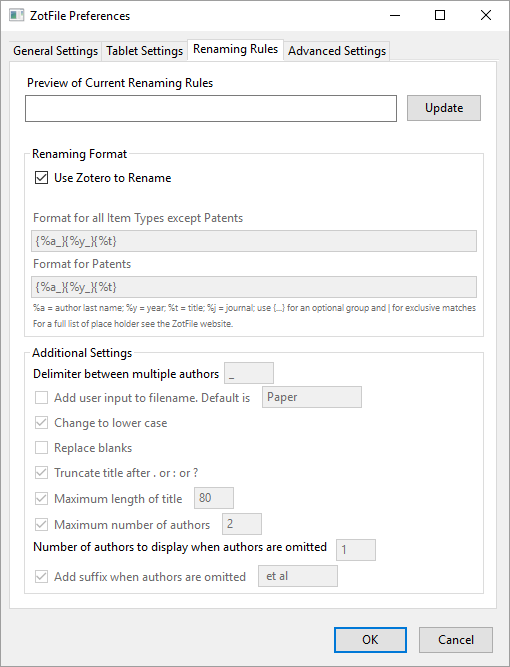
\includegraphics[height=3in, width = 4.25in,keepaspectratio]{zotero/zotfile_5.png}
\end{figure} \end{frame}

\section{Importing Citations}

\begin{frame} \frametitle{Citation 1: Find something you want to cite} \begin{figure}[!h] \centering
	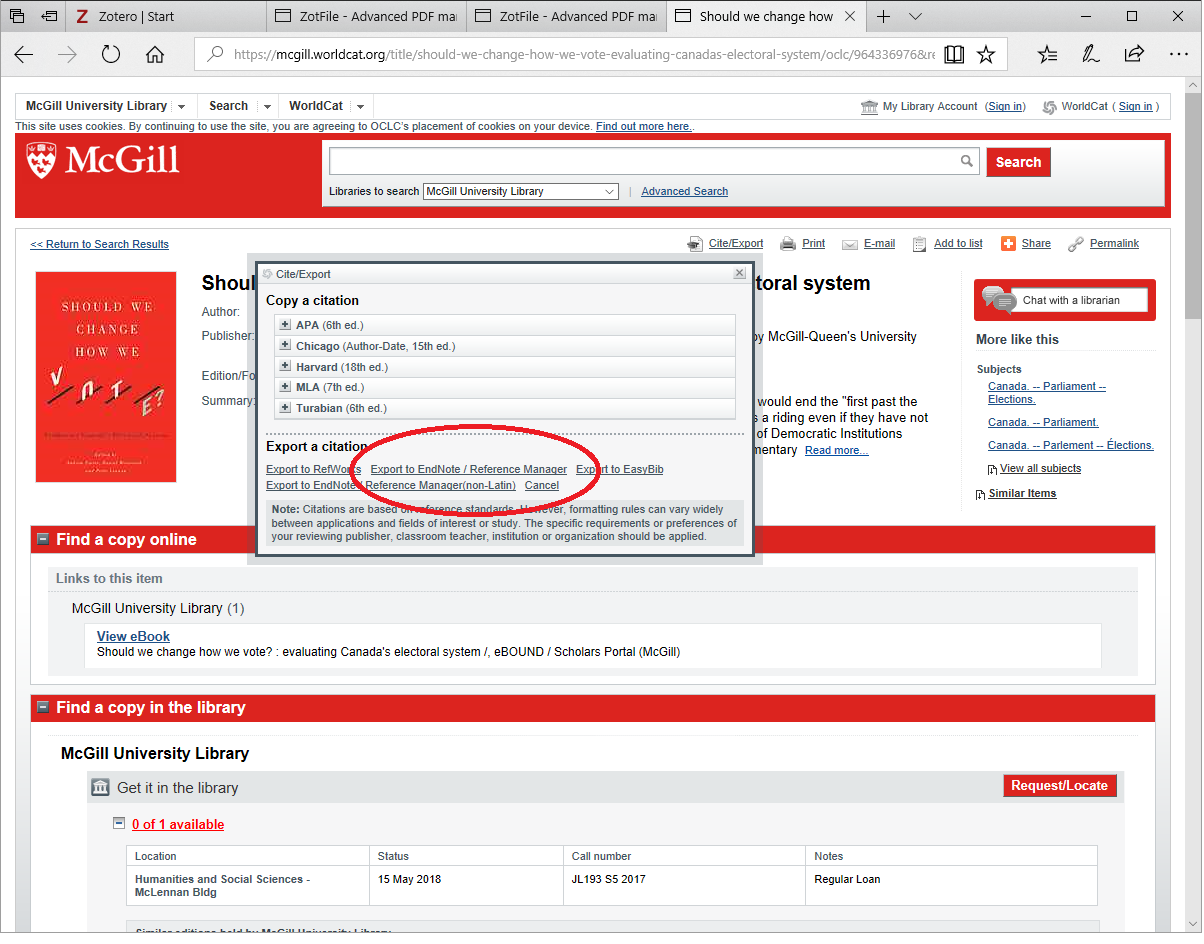
\includegraphics[height=3in, width = 4.25in,keepaspectratio]{zotero/citation_1.png}
\end{figure} \end{frame}

\begin{frame} \frametitle{Citation 2: Import into Zotero} \begin{figure}[!h] \centering
	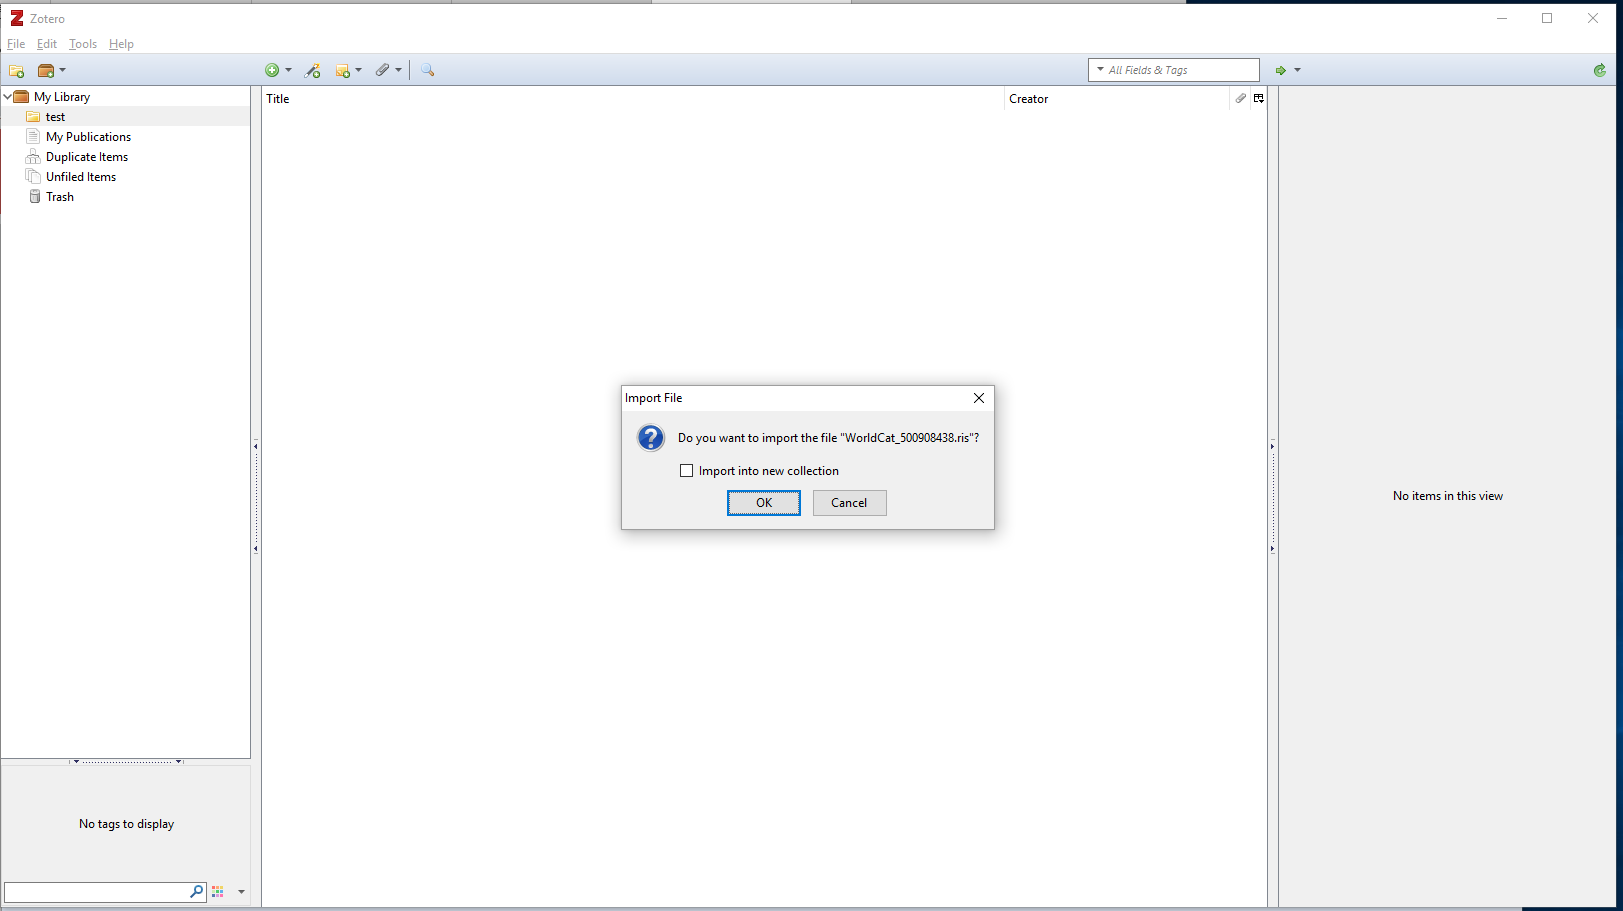
\includegraphics[height=3in, width = 4.25in,keepaspectratio]{zotero/citation_2.png}
\end{figure} \end{frame}

\begin{frame} \frametitle{Citation 3: Choose your fields} \begin{figure}[!h] \centering
	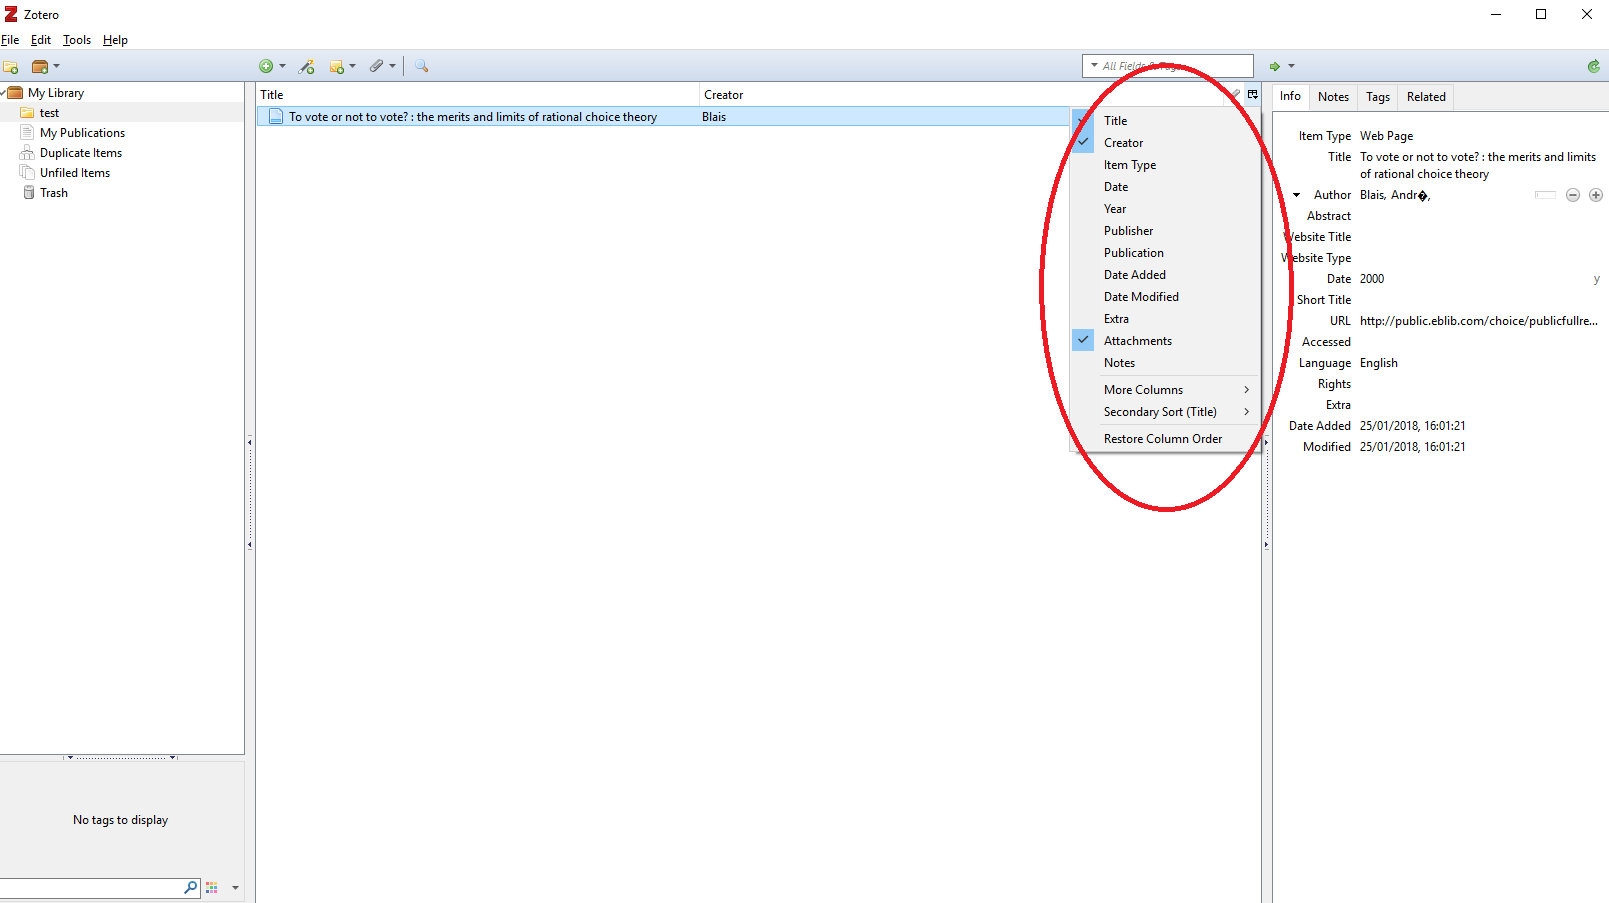
\includegraphics[height=3in, width = 4.25in,keepaspectratio]{zotero/citation_3.png}
\end{figure} \end{frame}

\begin{frame} \frametitle{Citation 4: Use google scholar} \begin{figure}[!h] \centering
	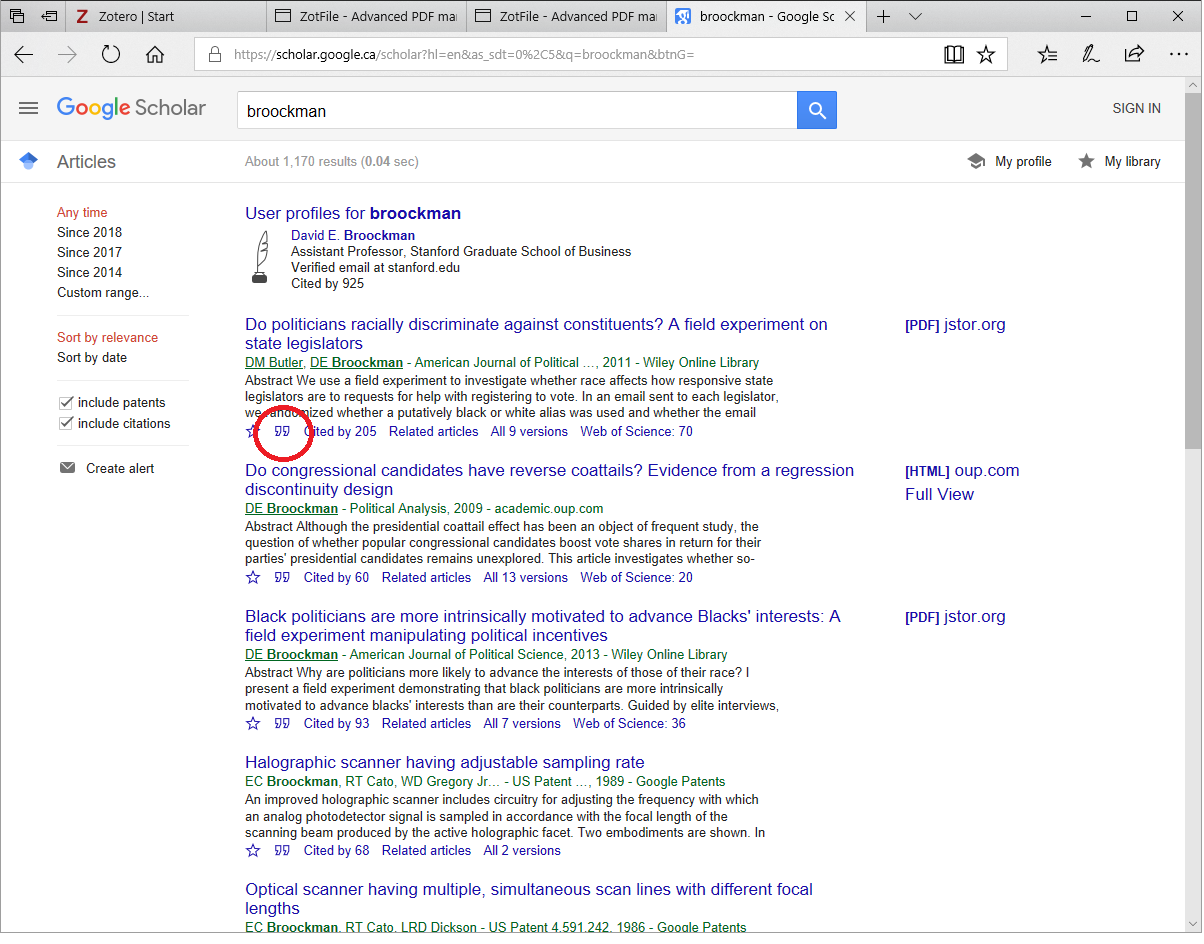
\includegraphics[height=3in, width = 4.25in,keepaspectratio]{zotero/citation_4.png}
\end{figure} \end{frame}

\begin{frame} \frametitle{Citation 5: Always use RefMan to get the .ris file} \begin{figure}[!h] \centering
	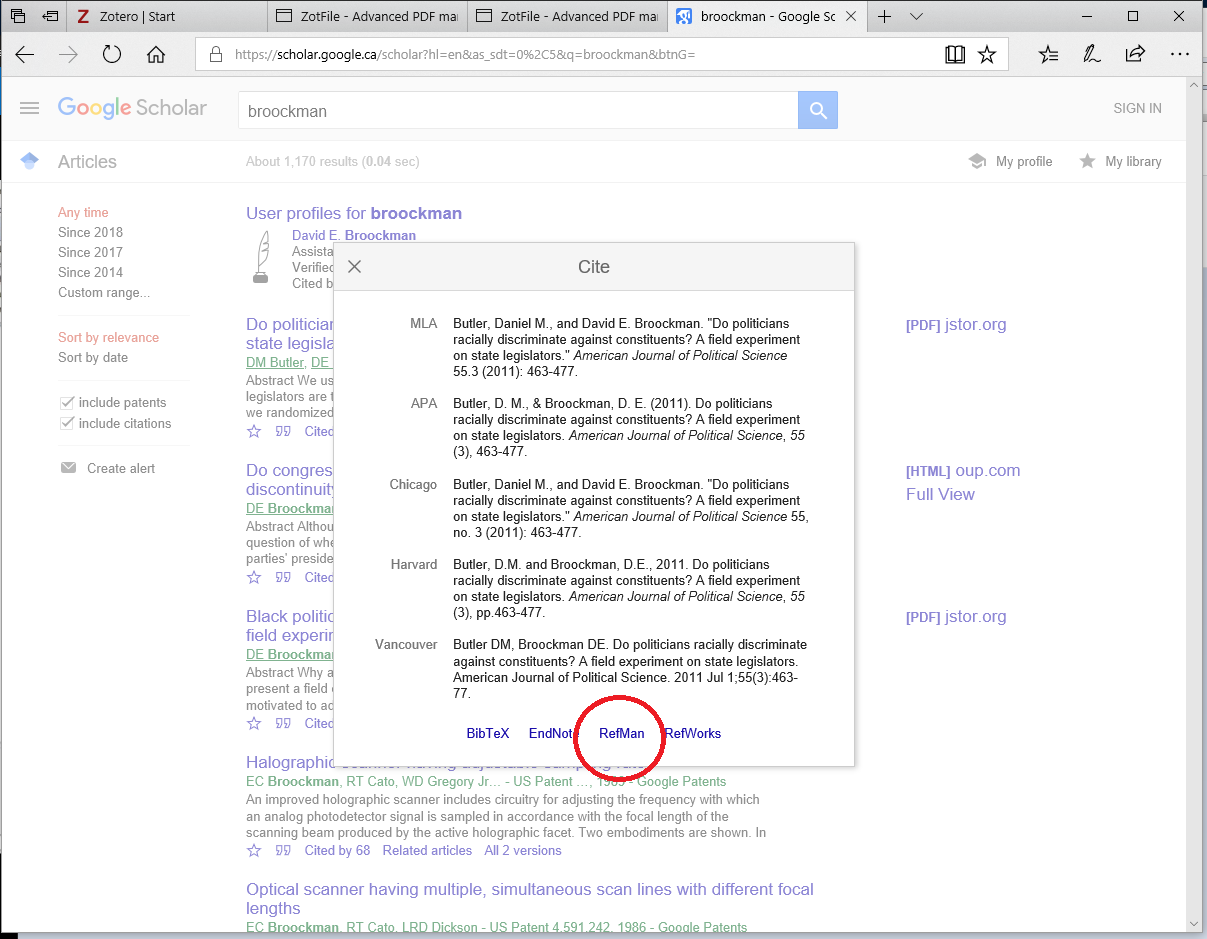
\includegraphics[height=3in, width = 4.25in,keepaspectratio]{zotero/citation_5.png}
\end{figure} \end{frame}

\begin{frame} \frametitle{Citation 6: Download the pdf} \begin{figure}[!h] \centering
	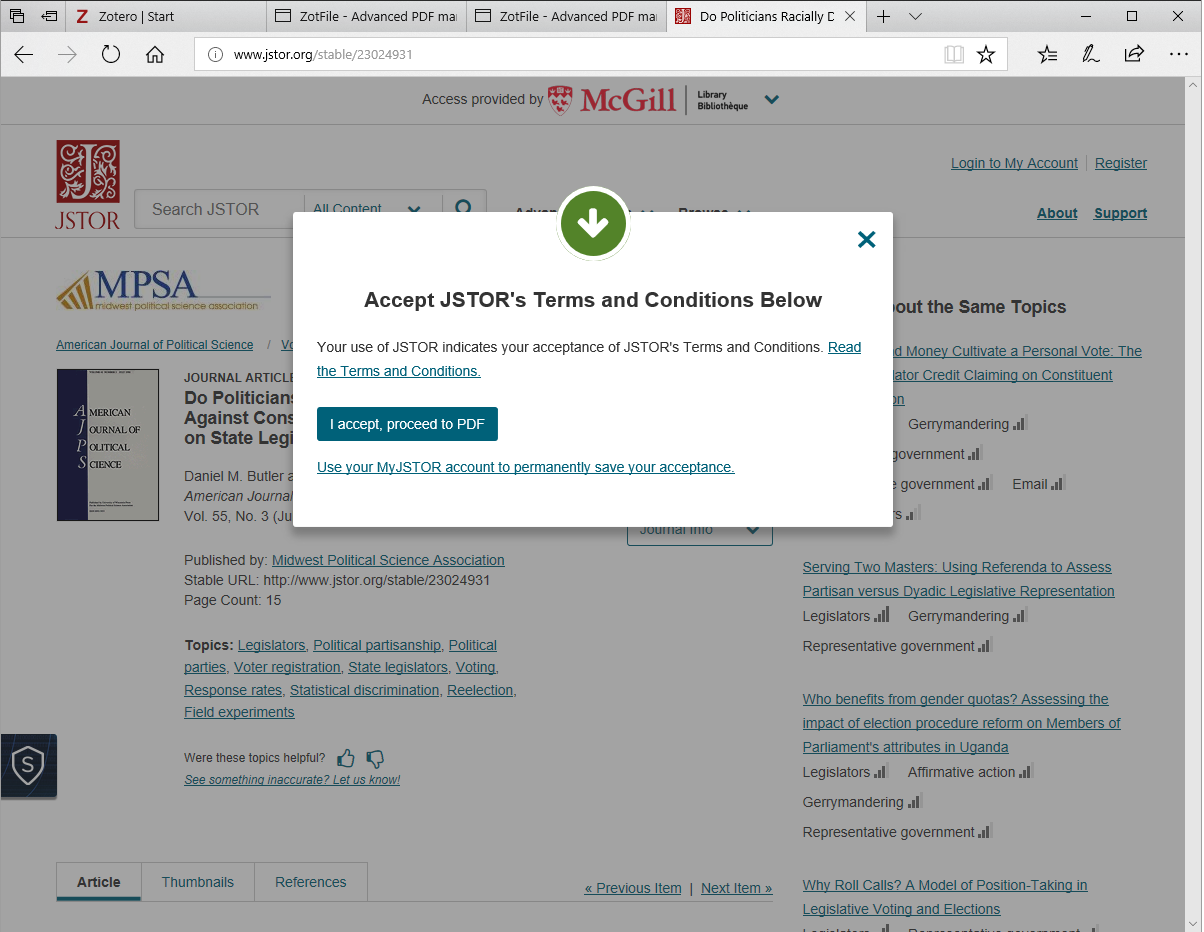
\includegraphics[height=3in, width = 4.25in,keepaspectratio]{zotero/citation_6.png}
\end{figure} \end{frame}

\begin{frame} \frametitle{Citation 7: Drag and drop} \begin{figure}[!h] \centering
	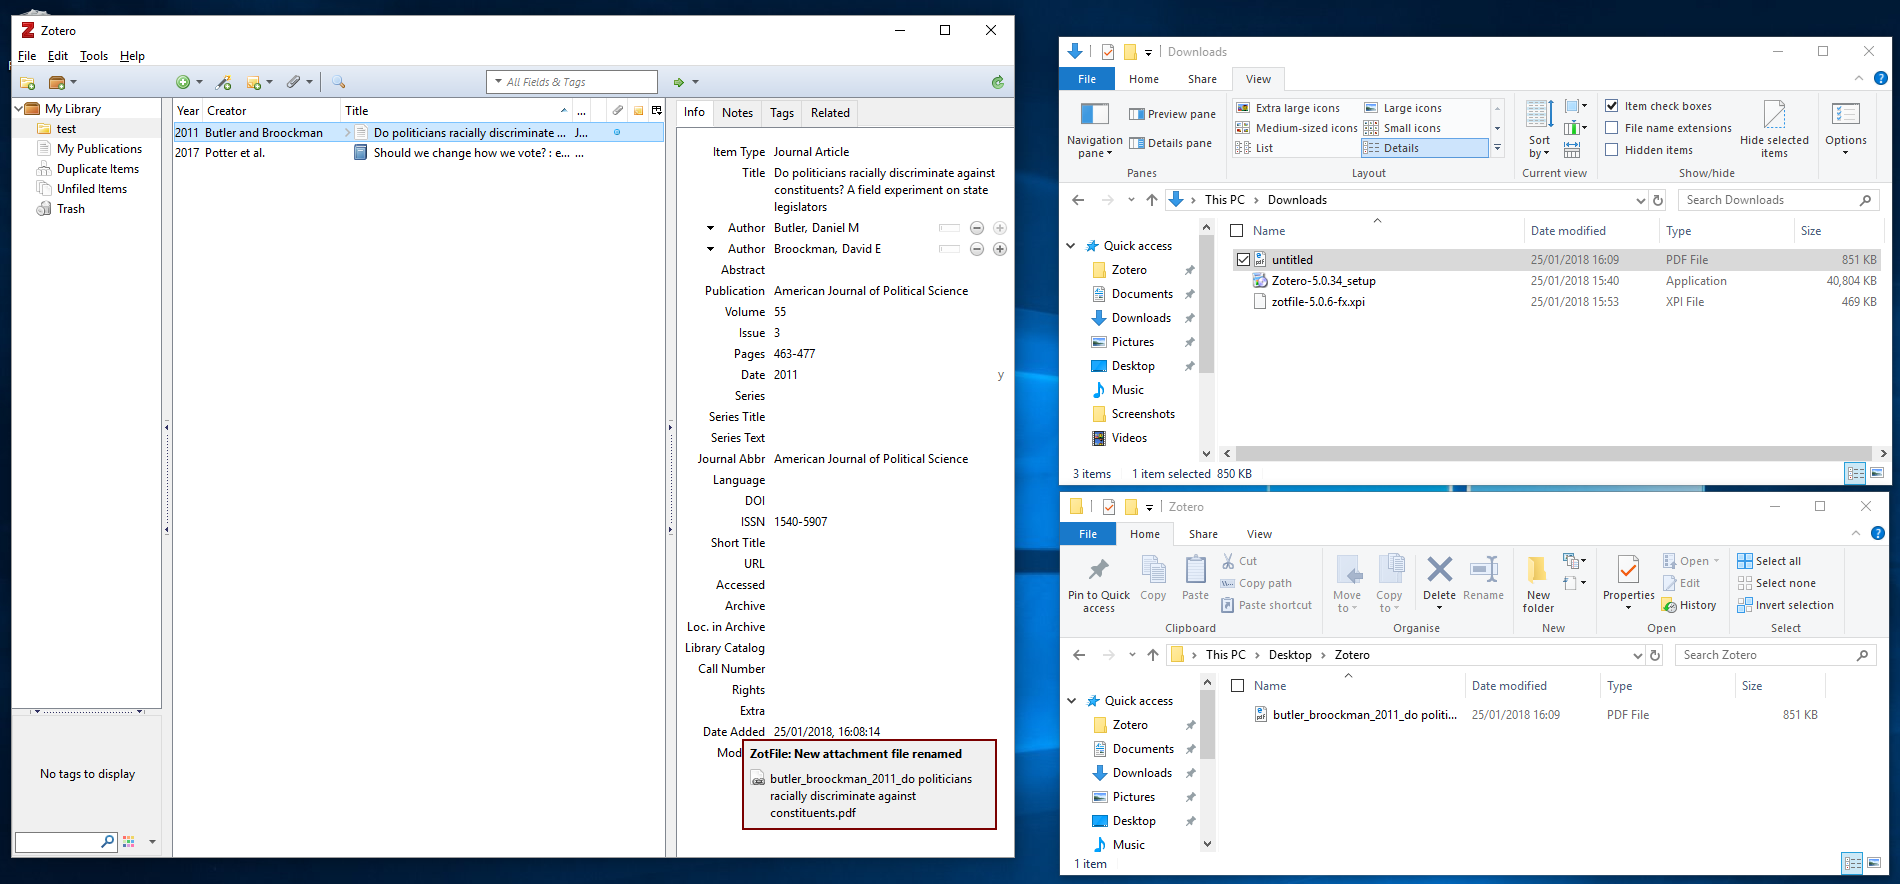
\includegraphics[height=3in, width = 4.25in,keepaspectratio]{zotero/citation_7.png}
\end{figure} \end{frame}

\section{Extracting information from PDFs}

\begin{frame} \frametitle{Extract 1: Put your pdf into Zotero} \begin{figure}[!h] \centering
	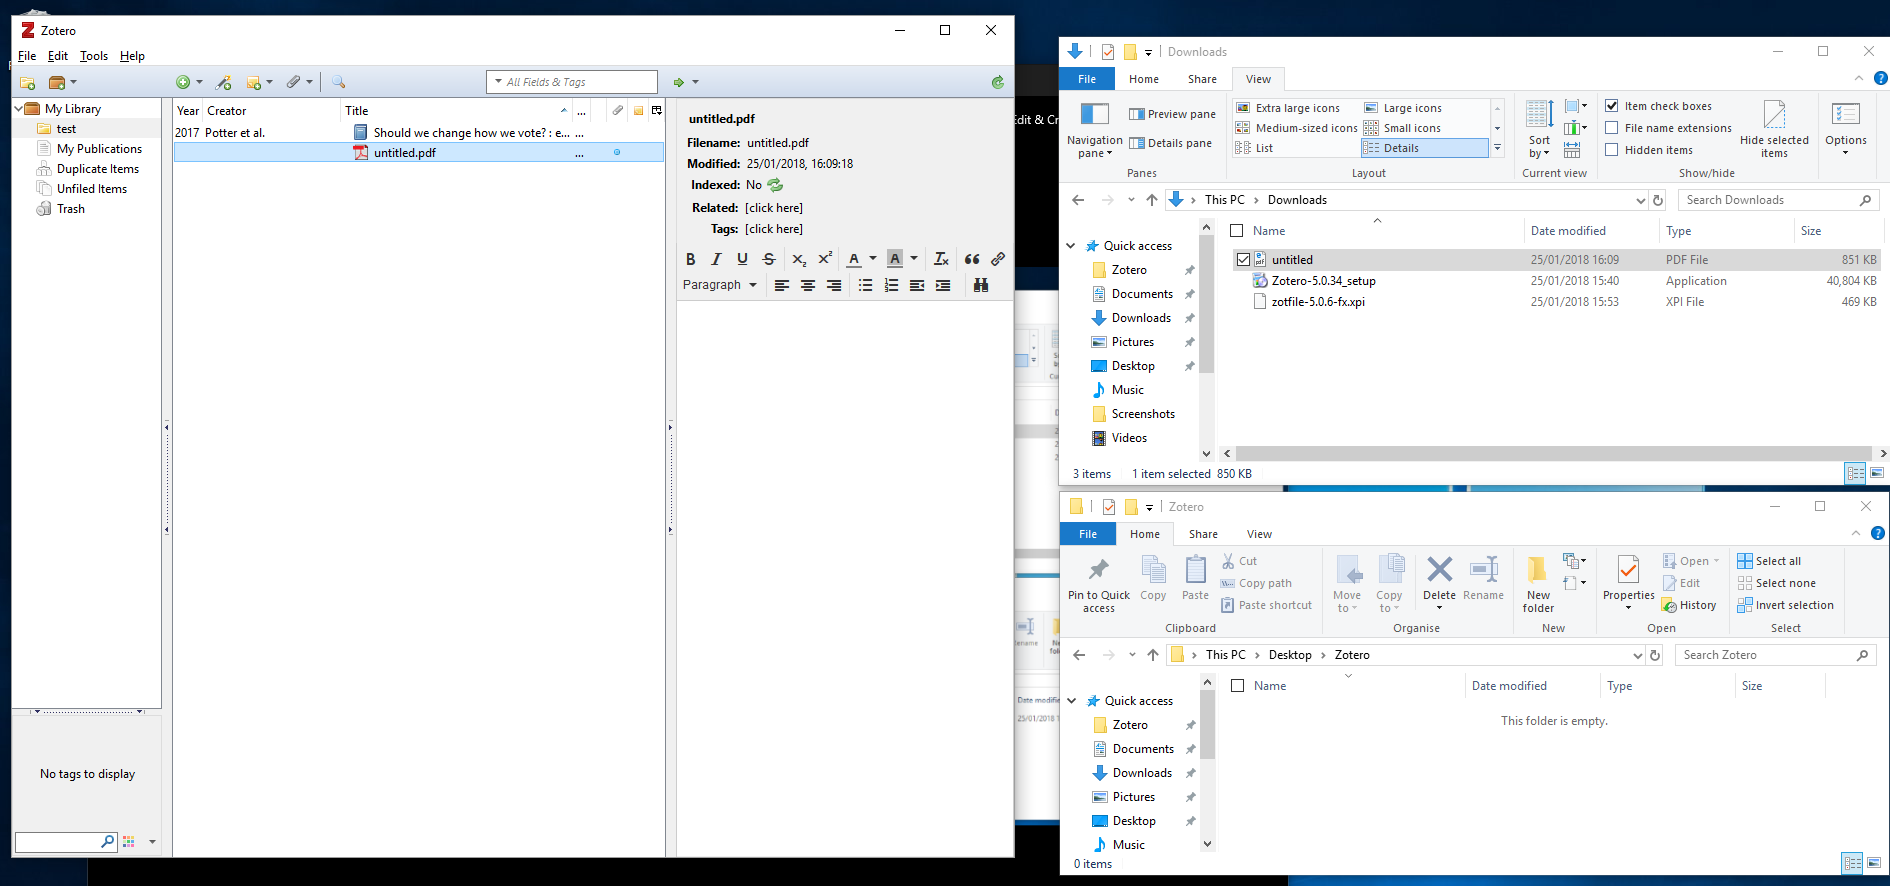
\includegraphics[height=3in, width = 4.25in,keepaspectratio]{zotero/extract_1.png}
\end{figure} \end{frame}

\begin{frame} \frametitle{Extract 2: Retrieve metadata} \begin{figure}[!h] \centering
	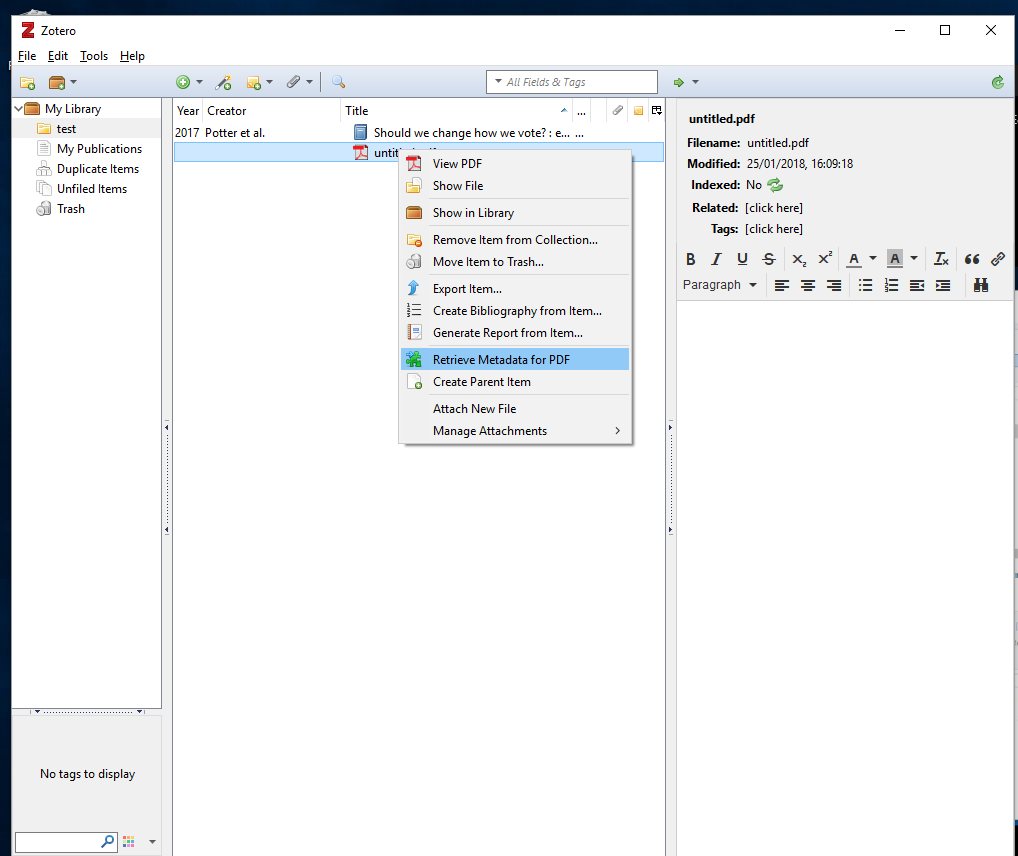
\includegraphics[height=3in, width = 4.25in,keepaspectratio]{zotero/extract_2.png}
\end{figure} \end{frame}

\begin{frame} \frametitle{Extract 3: Install PDF Indexing} \begin{figure}[!h] \centering
	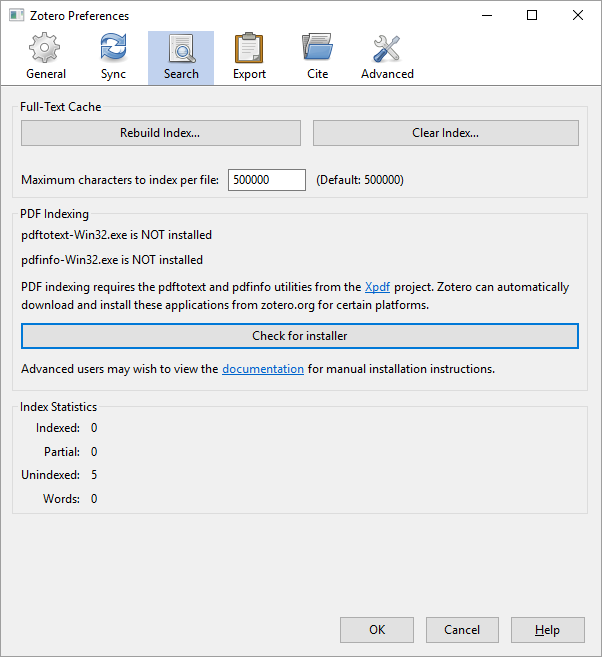
\includegraphics[height=3in, width = 4.25in,keepaspectratio]{zotero/extract_3.png}
\end{figure} \end{frame}

\begin{frame} \frametitle{Extract 4: Success!} \begin{figure}[!h] \centering
	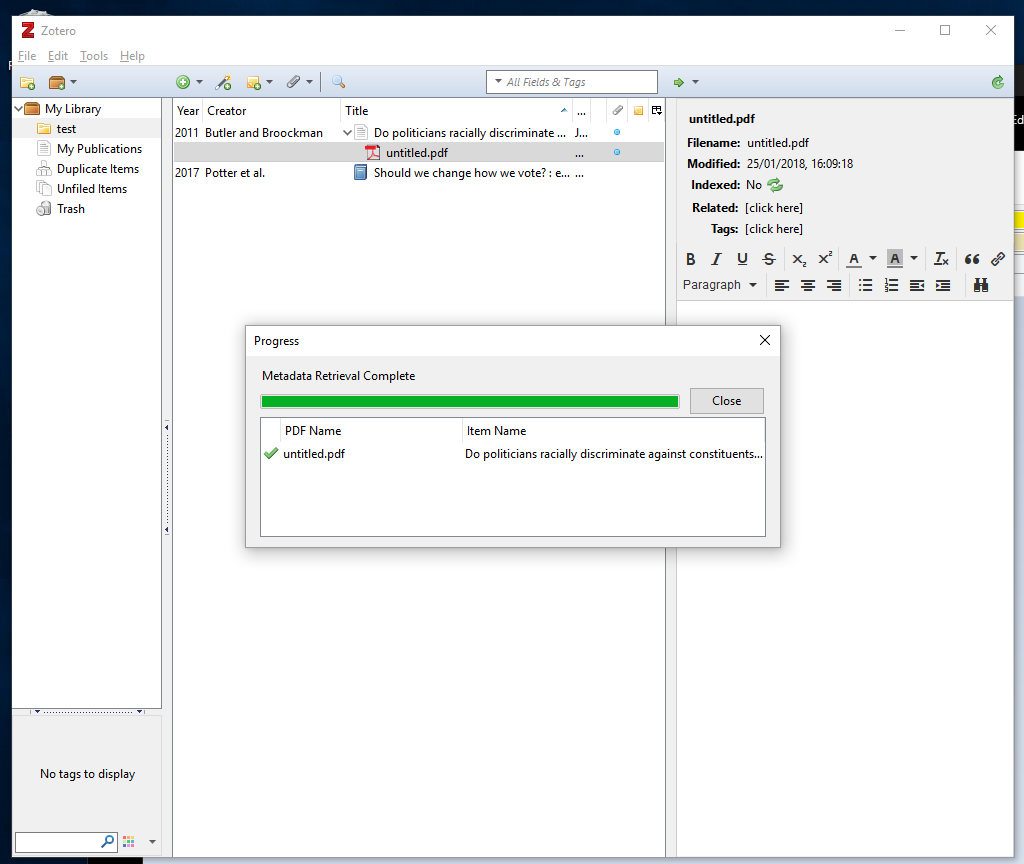
\includegraphics[height=3in, width = 4.25in,keepaspectratio]{zotero/extract_4.png}
\end{figure} \end{frame}

\begin{frame} \frametitle{Extract 5: Rename Attachments} \begin{figure}[!h] \centering
	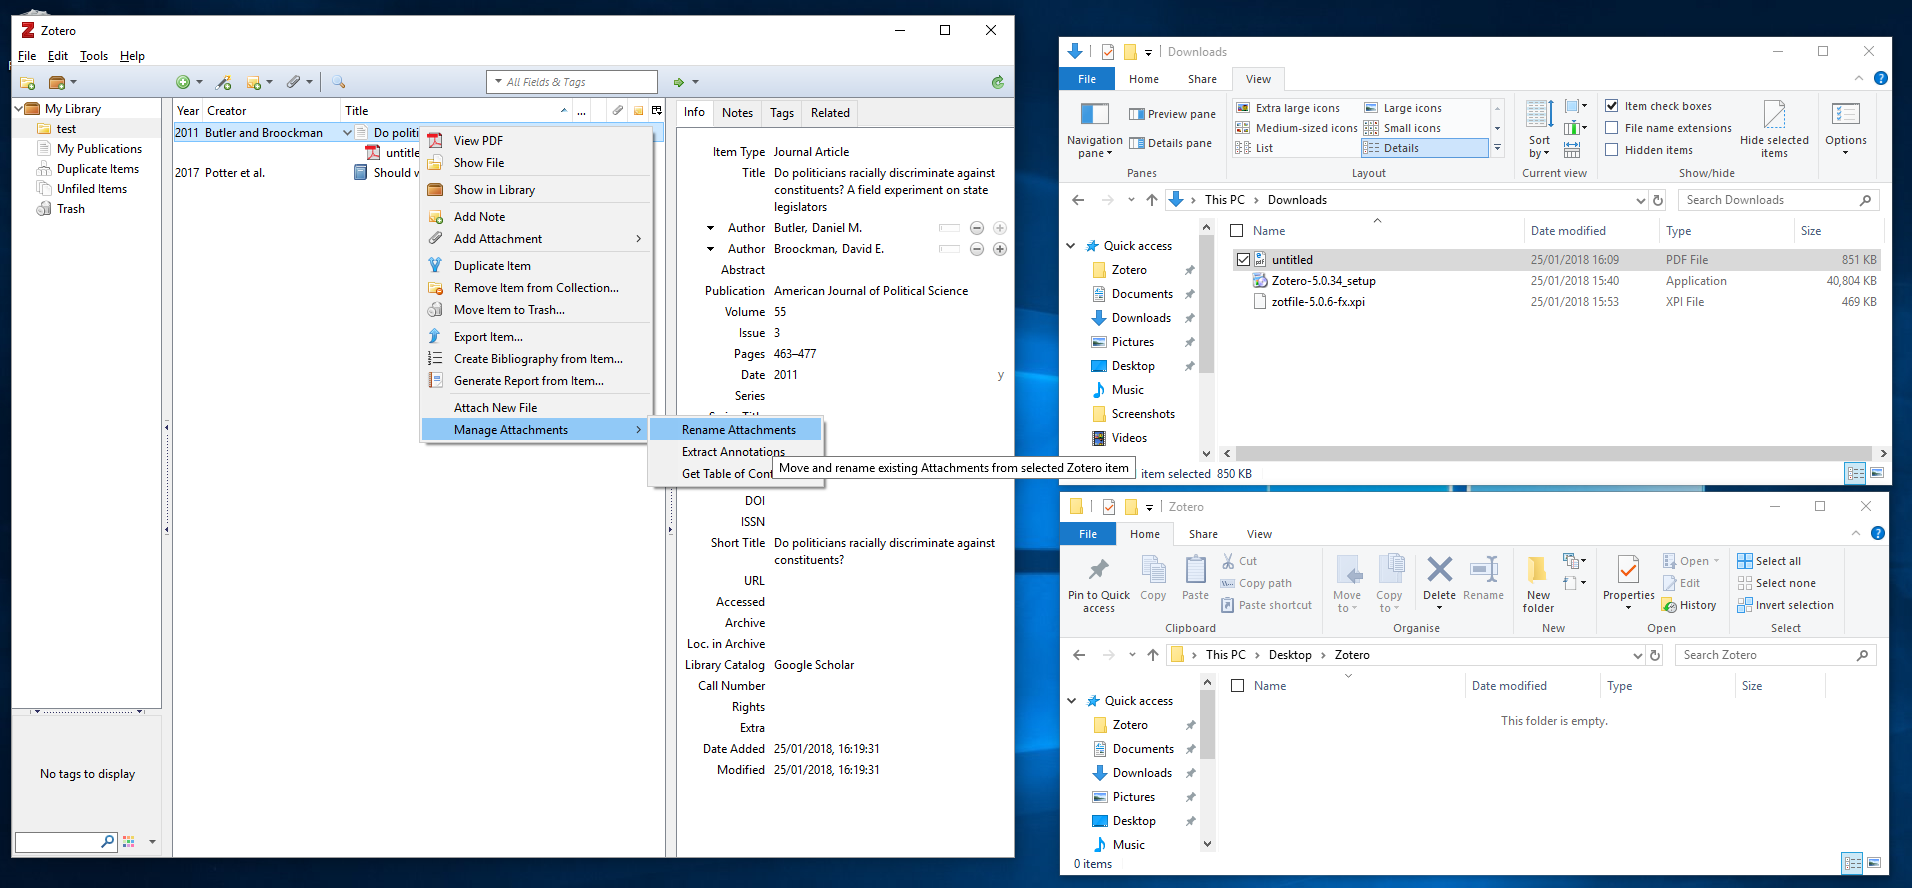
\includegraphics[height=3in, width = 4.25in,keepaspectratio]{zotero/extract_5.png}
\end{figure} \end{frame}

\begin{frame} \frametitle{Extract 6: Now it is in your central location!} \begin{figure}[!h] \centering
	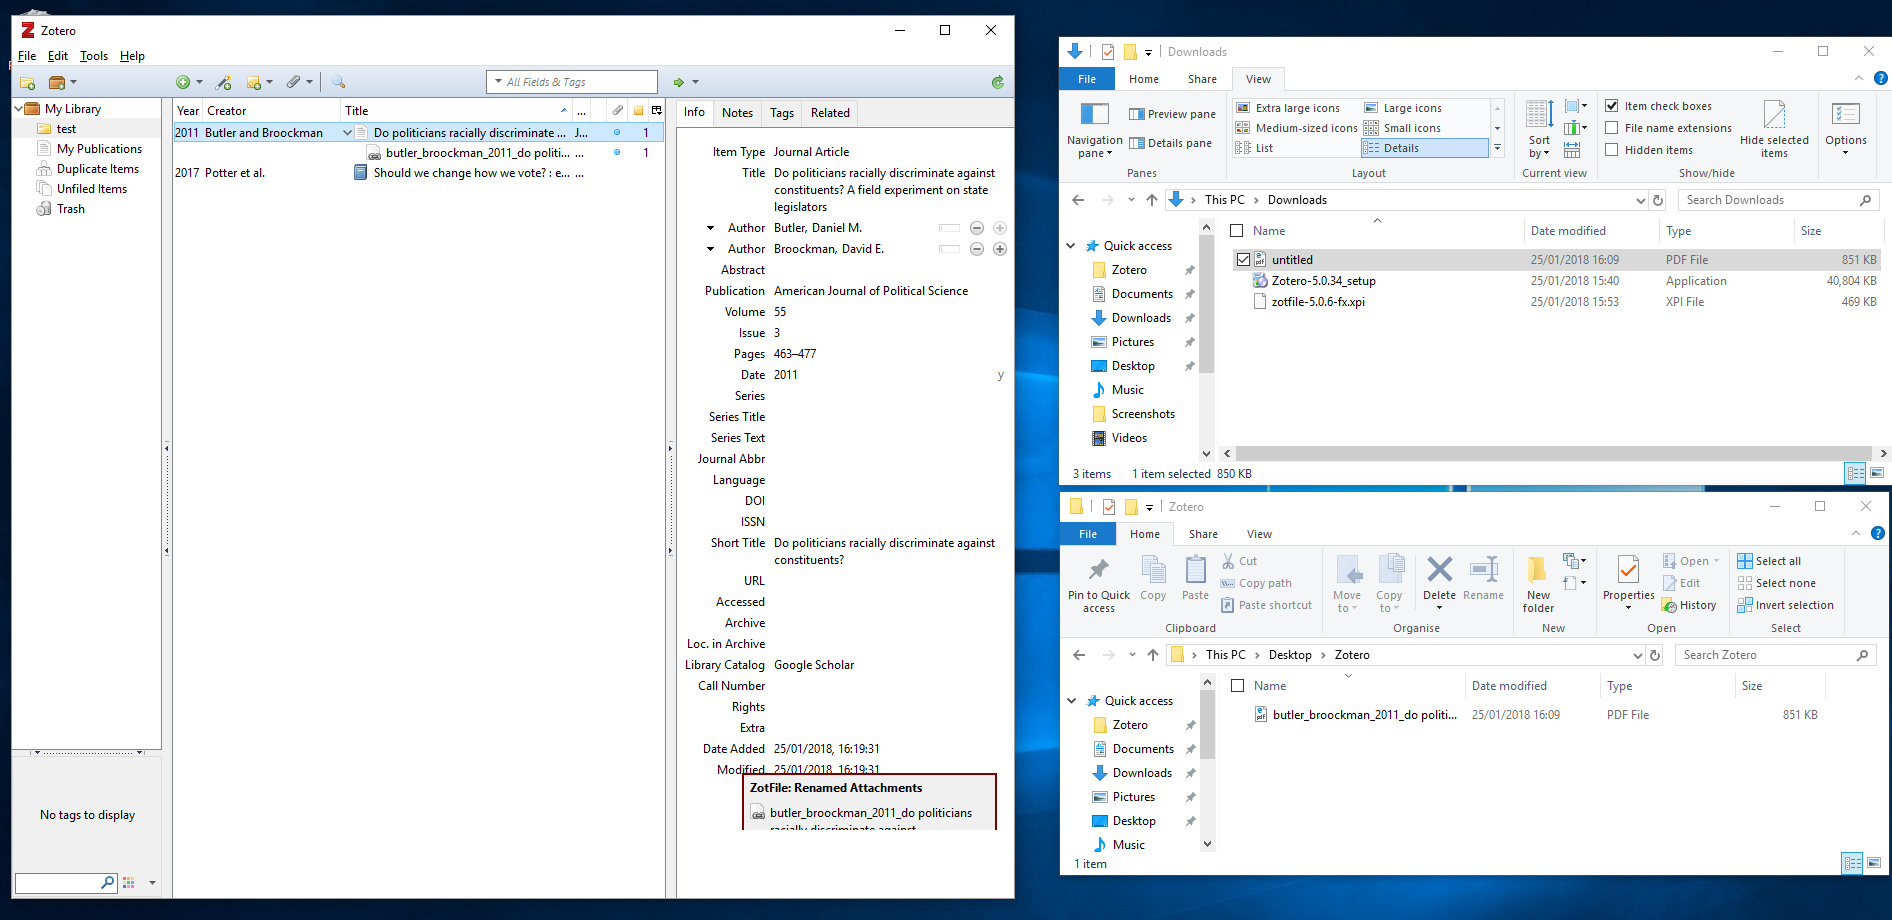
\includegraphics[height=3in, width = 4.25in,keepaspectratio]{zotero/extract_6.png}
\end{figure} \end{frame}

\section{Time to integrate with Microsoft Word}

\begin{frame} \frametitle{Word 1: Should have Zotero add-in already installed} \begin{figure}[!h] \centering
	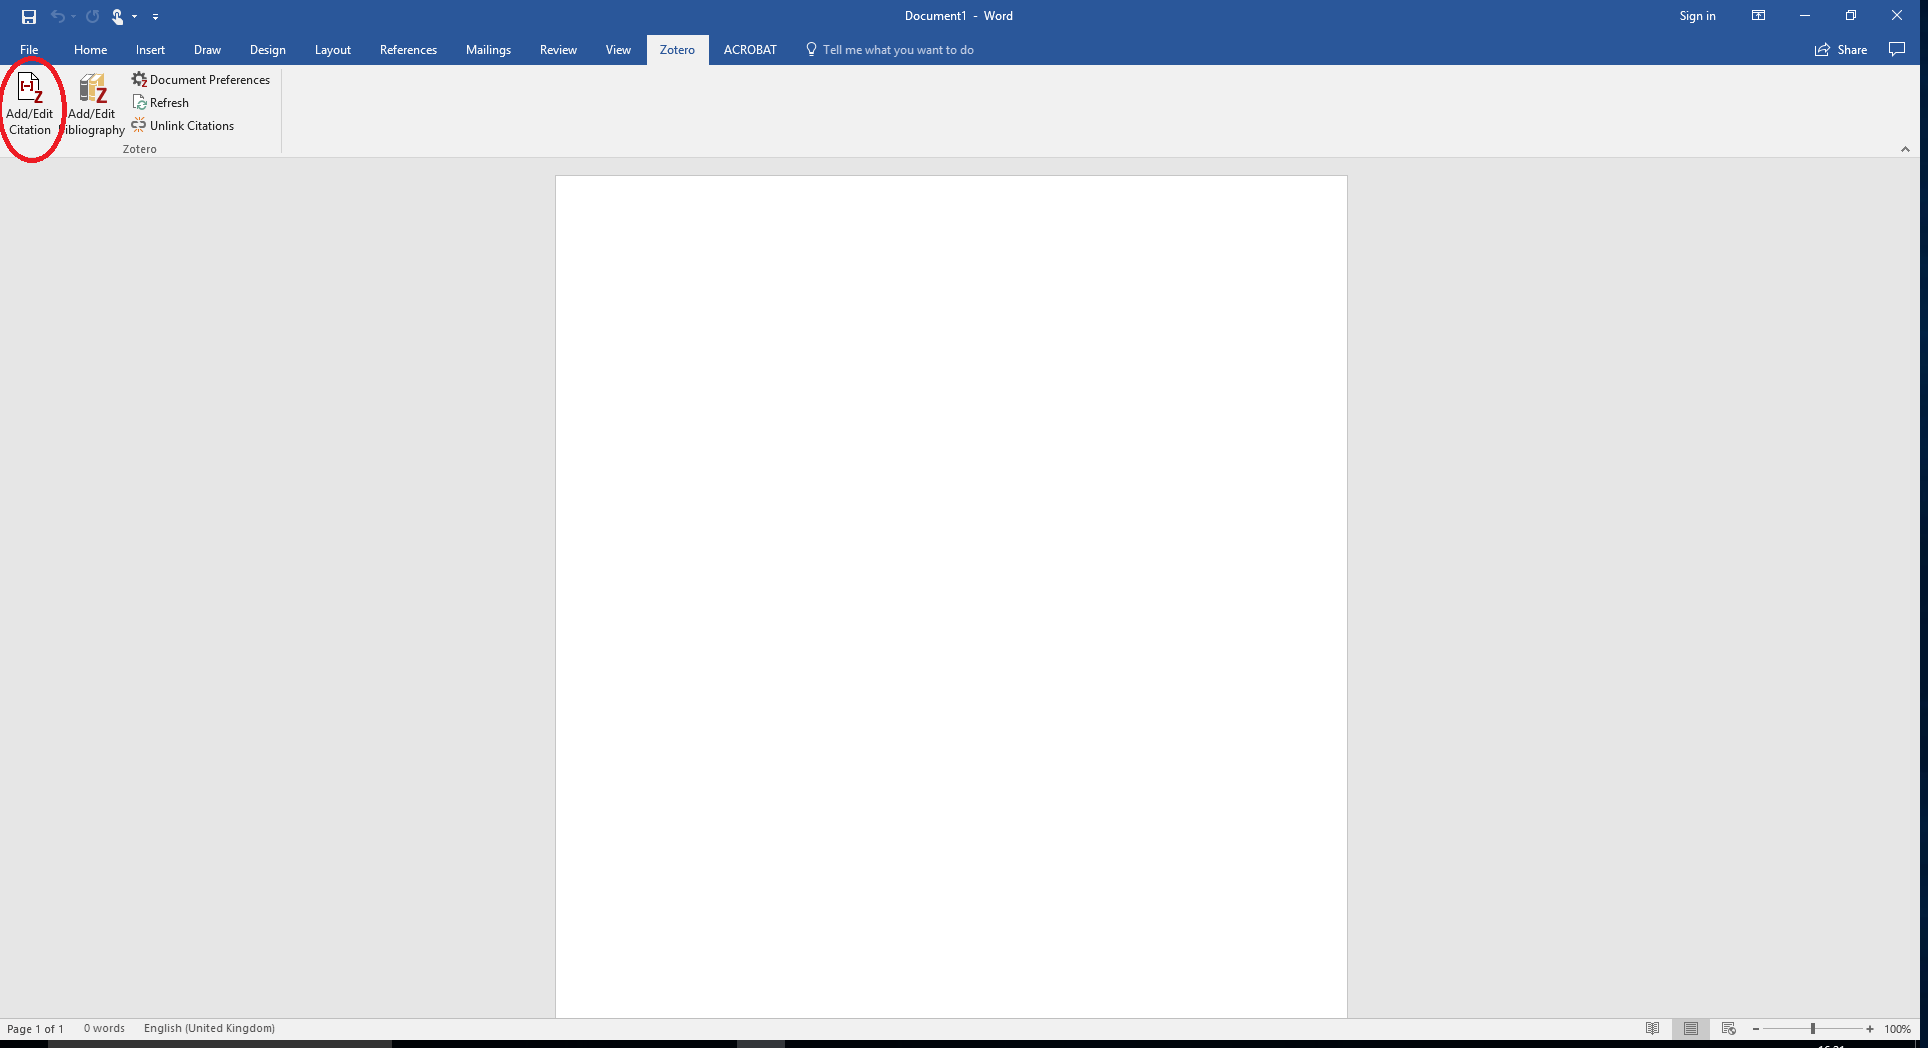
\includegraphics[height=3in, width = 4.25in,keepaspectratio]{zotero/word_1.png}
\end{figure} \end{frame}

\begin{frame} \frametitle{Word 2: Choose your citation style} \begin{figure}[!h] \centering
	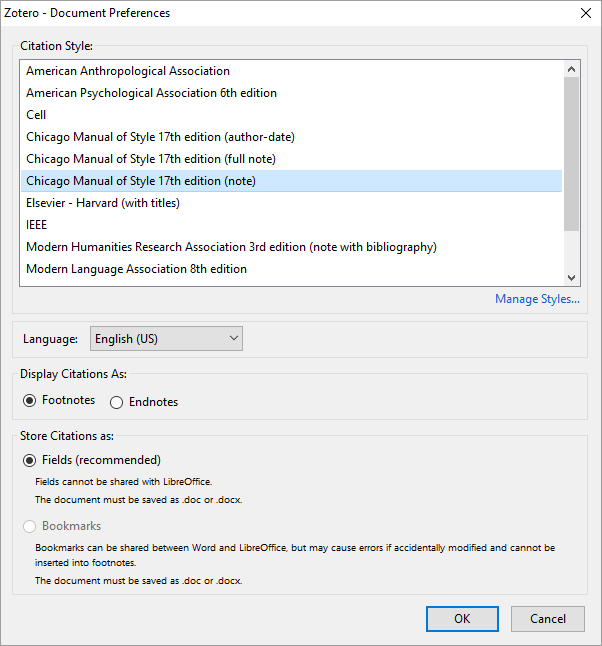
\includegraphics[height=3in, width = 4.25in,keepaspectratio]{zotero/word_2.png}
\end{figure} \end{frame}

\begin{frame} \frametitle{Word 3: Type of a few letters...} \begin{figure}[!h] \centering
	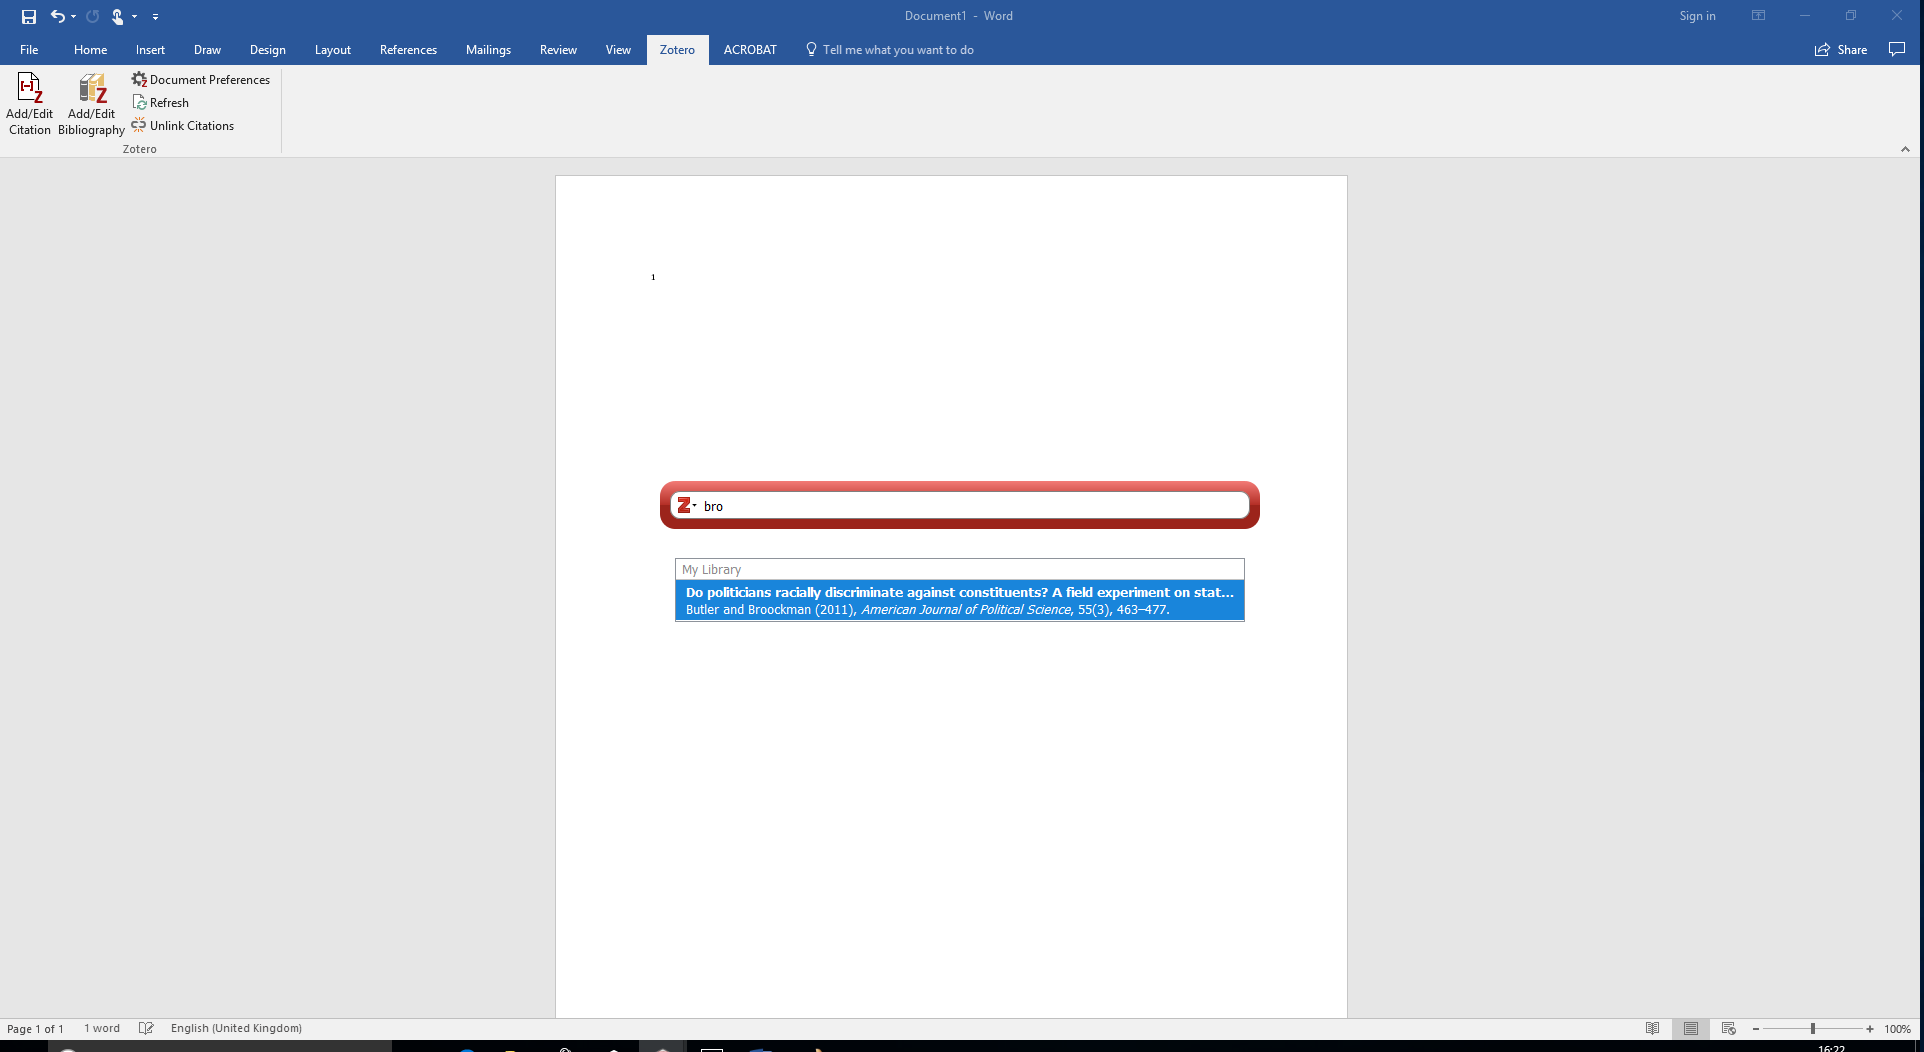
\includegraphics[height=3in, width = 4.25in,keepaspectratio]{zotero/word_3.png}
\end{figure} \end{frame}

\begin{frame} \frametitle{Word 4: Let's set a shortcut in Options} \begin{figure}[!h] \centering
	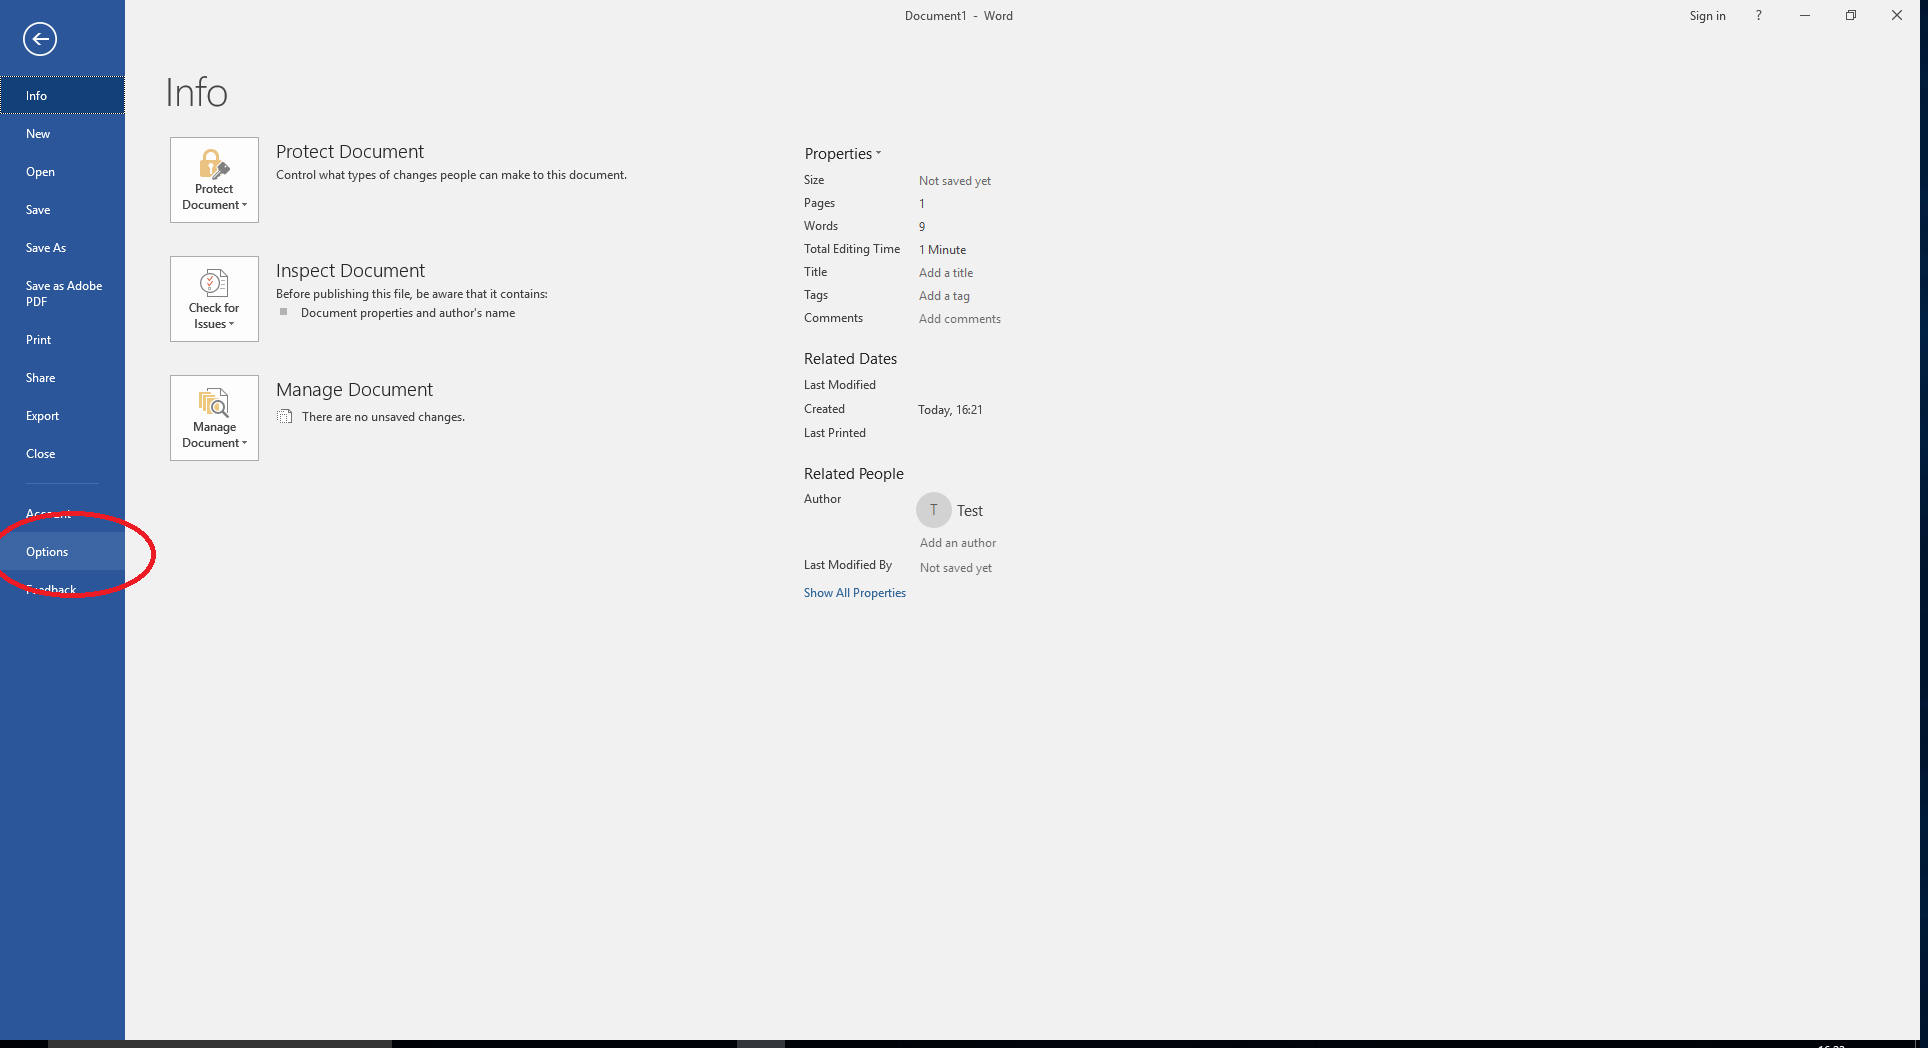
\includegraphics[height=3in, width = 4.25in,keepaspectratio]{zotero/word_4.png}
\end{figure} \end{frame}

\begin{frame} \frametitle{Word 5: Keyboard shortcut customize} \begin{figure}[!h] \centering
	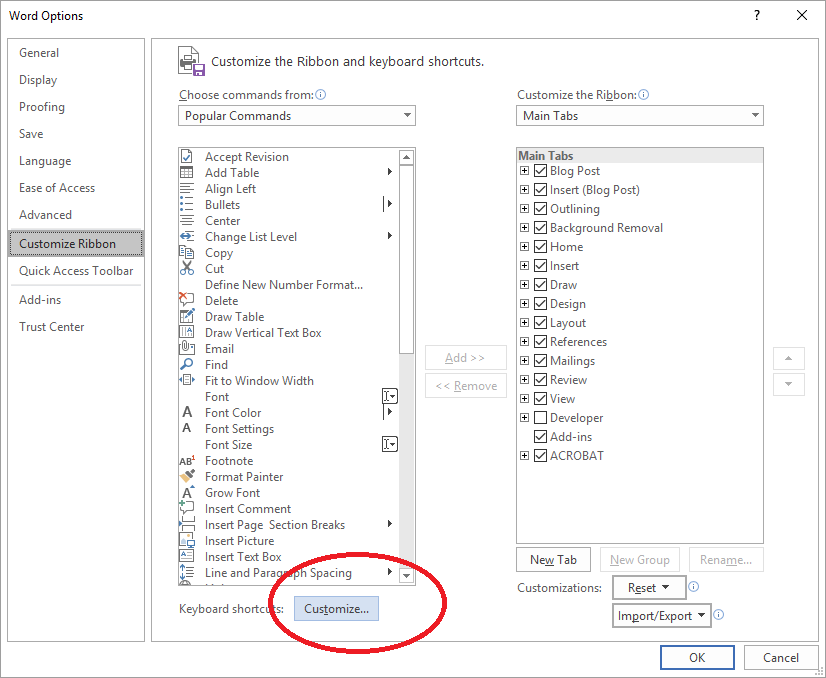
\includegraphics[height=3in, width = 4.25in,keepaspectratio]{zotero/word_5.png}
\end{figure} \end{frame}

\begin{frame} \frametitle{Word 6: Find Macros} \begin{figure}[!h] \centering
	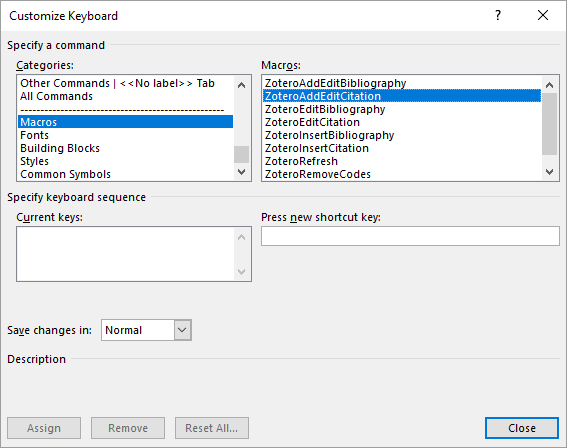
\includegraphics[height=3in, width = 4.25in,keepaspectratio]{zotero/word_6.png}
\end{figure} \end{frame}

\begin{frame} \frametitle{Word 7: Assign!} \begin{figure}[!h] \centering
	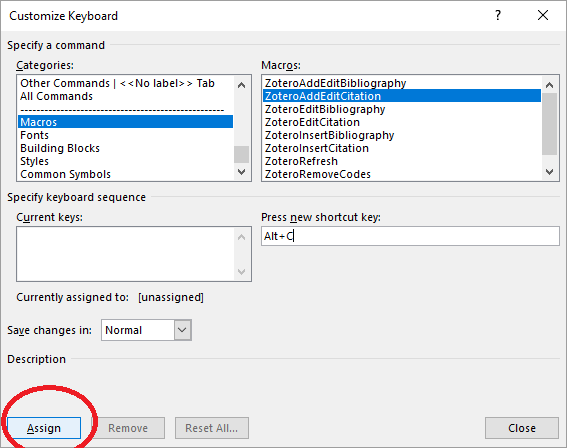
\includegraphics[height=3in, width = 4.25in,keepaspectratio]{zotero/word_7.png}
\end{figure} \end{frame}

\section{Time to create a .bib file with all the references}

\begin{frame} \frametitle{Bib 1: Install better bibtex} \begin{figure}[!h] \centering
	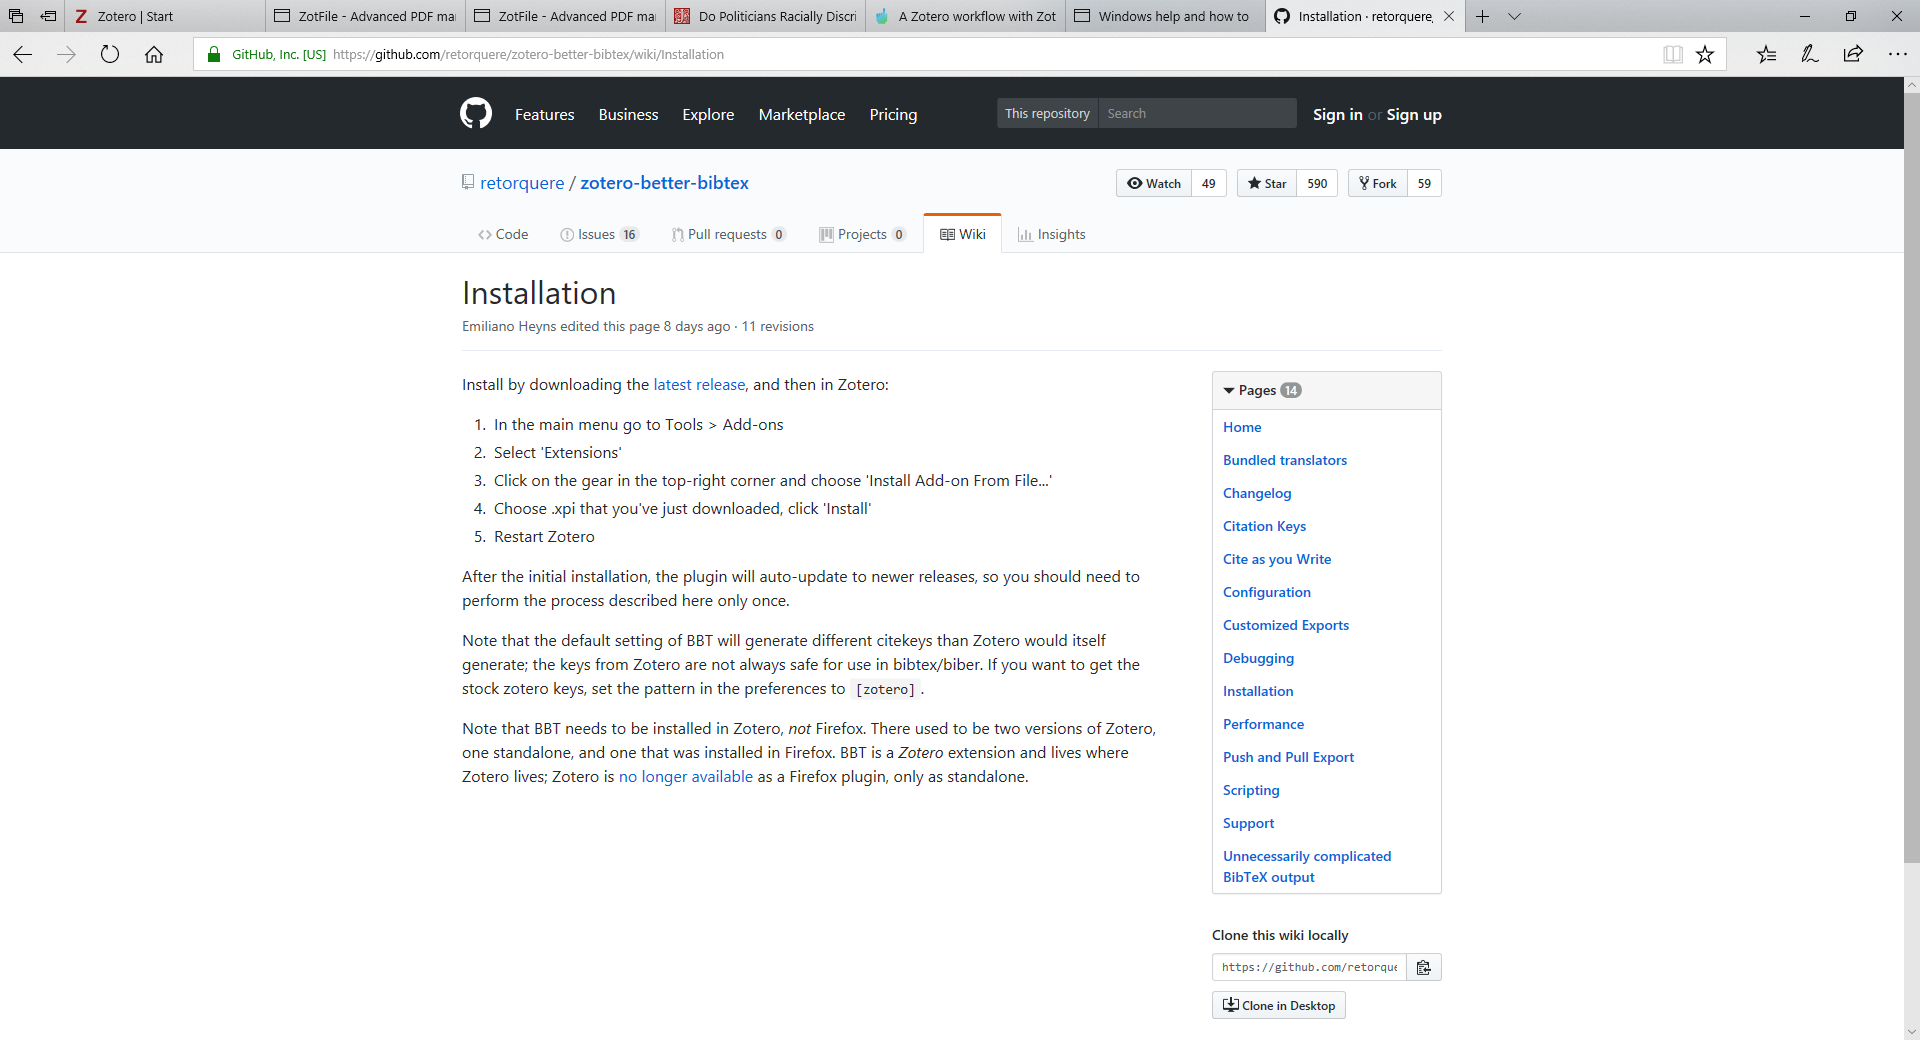
\includegraphics[height=3in, width = 4.25in,keepaspectratio]{zotero/bibtex_1.png}
\end{figure} \end{frame}

\begin{frame} \frametitle{Bib 2: Installing an add-in} \begin{figure}[!h] \centering
	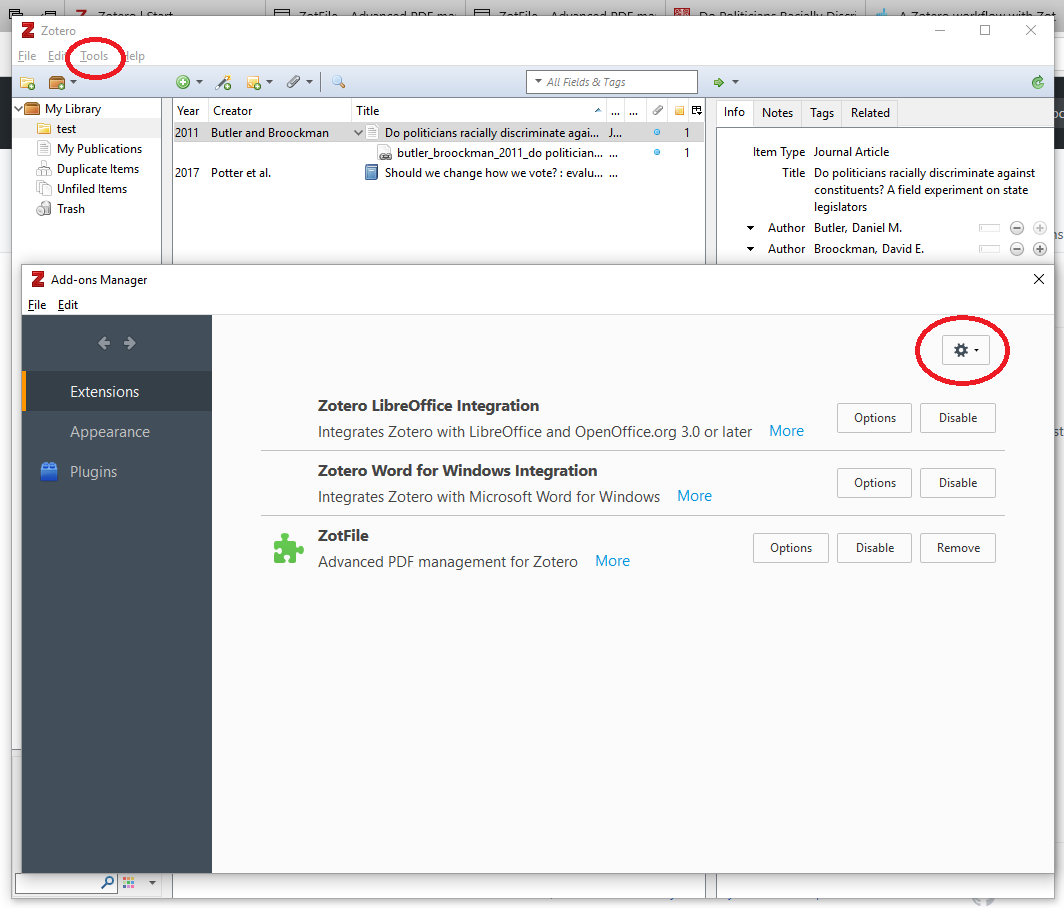
\includegraphics[height=3in, width = 4.25in,keepaspectratio]{zotero/bibtex_2.png}
\end{figure} \end{frame}

\begin{frame} \frametitle{Bib 3: Find your new file} \begin{figure}[!h] \centering
	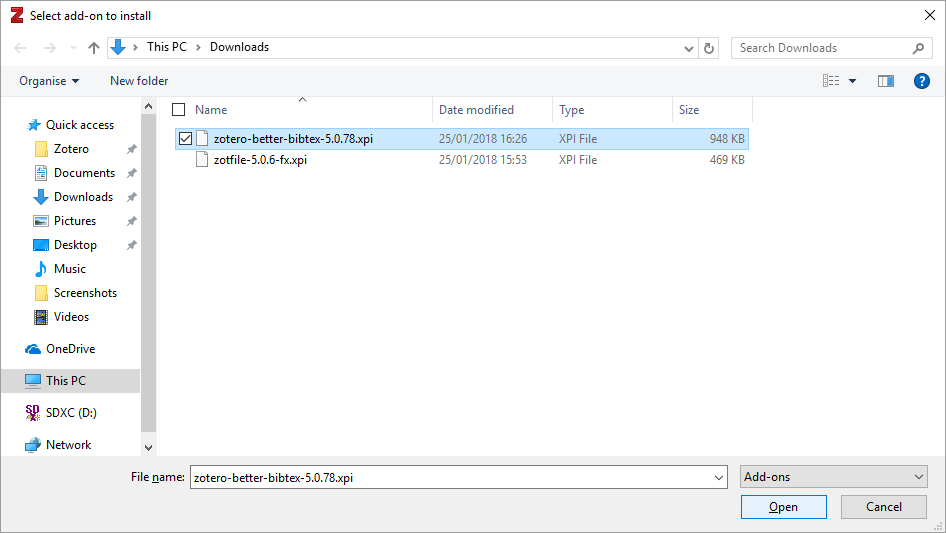
\includegraphics[height=3in, width = 4.25in,keepaspectratio]{zotero/bibtex_3.png}
\end{figure} \end{frame}

\begin{frame} \frametitle{Bib 4: Select your option, but can change later} \begin{figure}[!h] \centering
	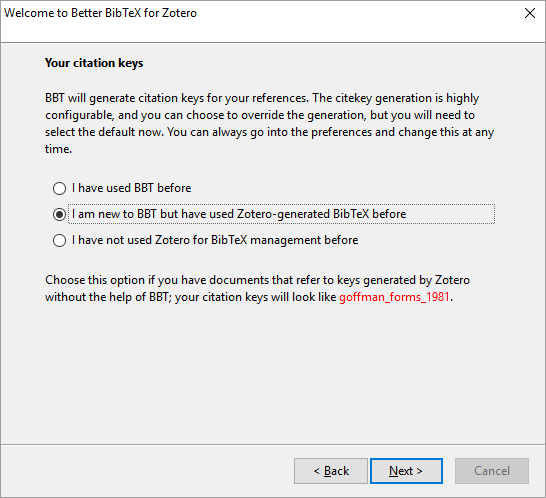
\includegraphics[height=3in, width = 4.25in,keepaspectratio]{zotero/bibtex_4.png}
\end{figure} \end{frame}

\begin{frame} \frametitle{Bib 5: Aha! A citation key} \begin{figure}[!h] \centering
	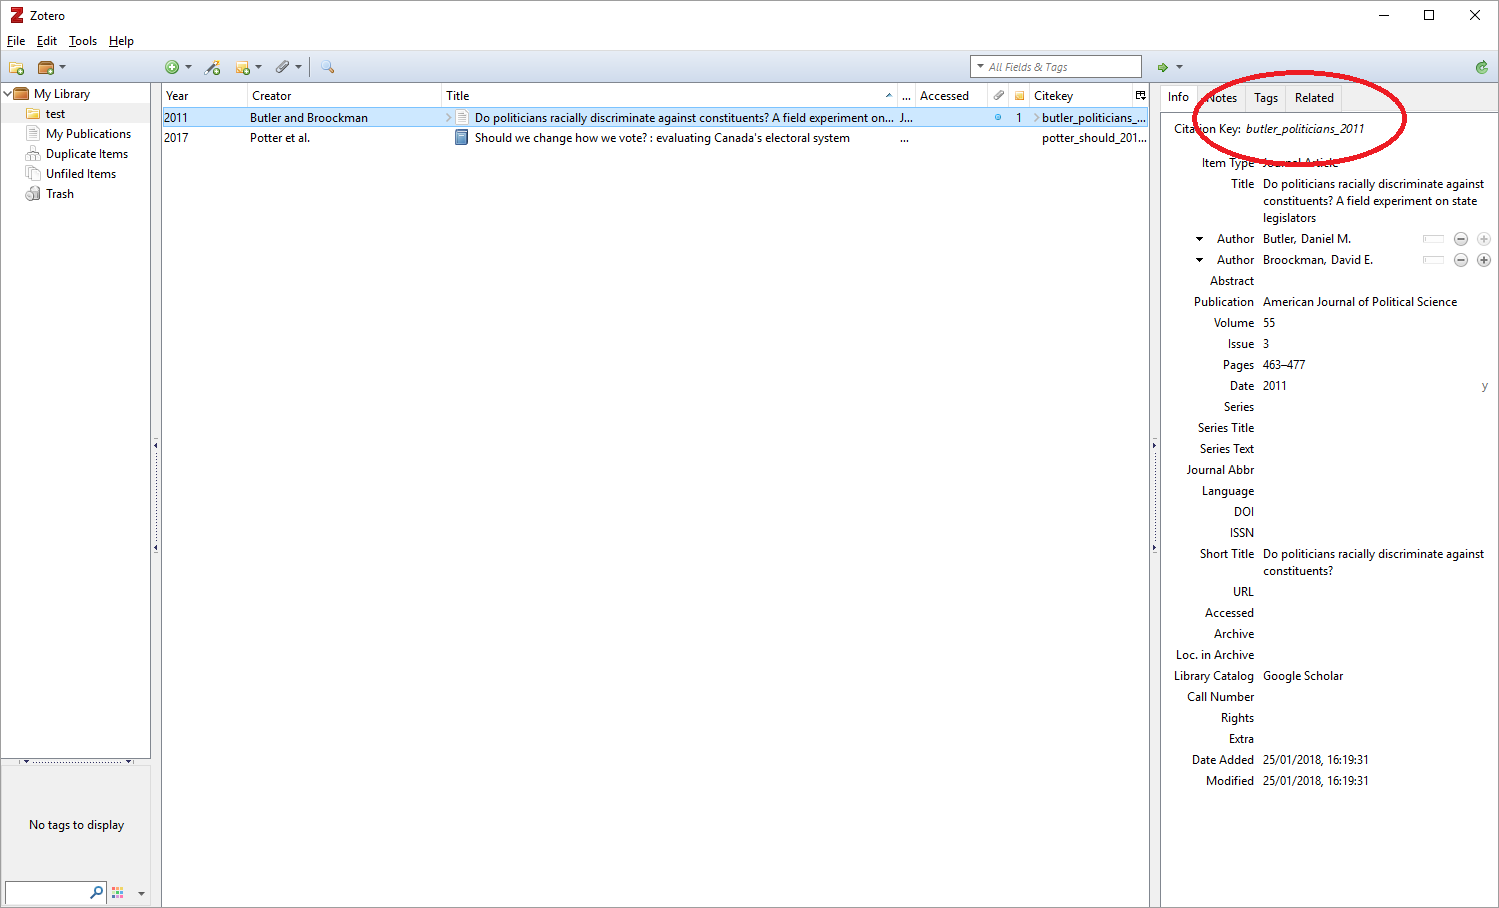
\includegraphics[height=3in, width = 4.25in,keepaspectratio]{zotero/bibtex_5.png}
\end{figure} \end{frame}

\begin{frame} \frametitle{Bib 6: Export Library} \begin{figure}[!h] \centering
	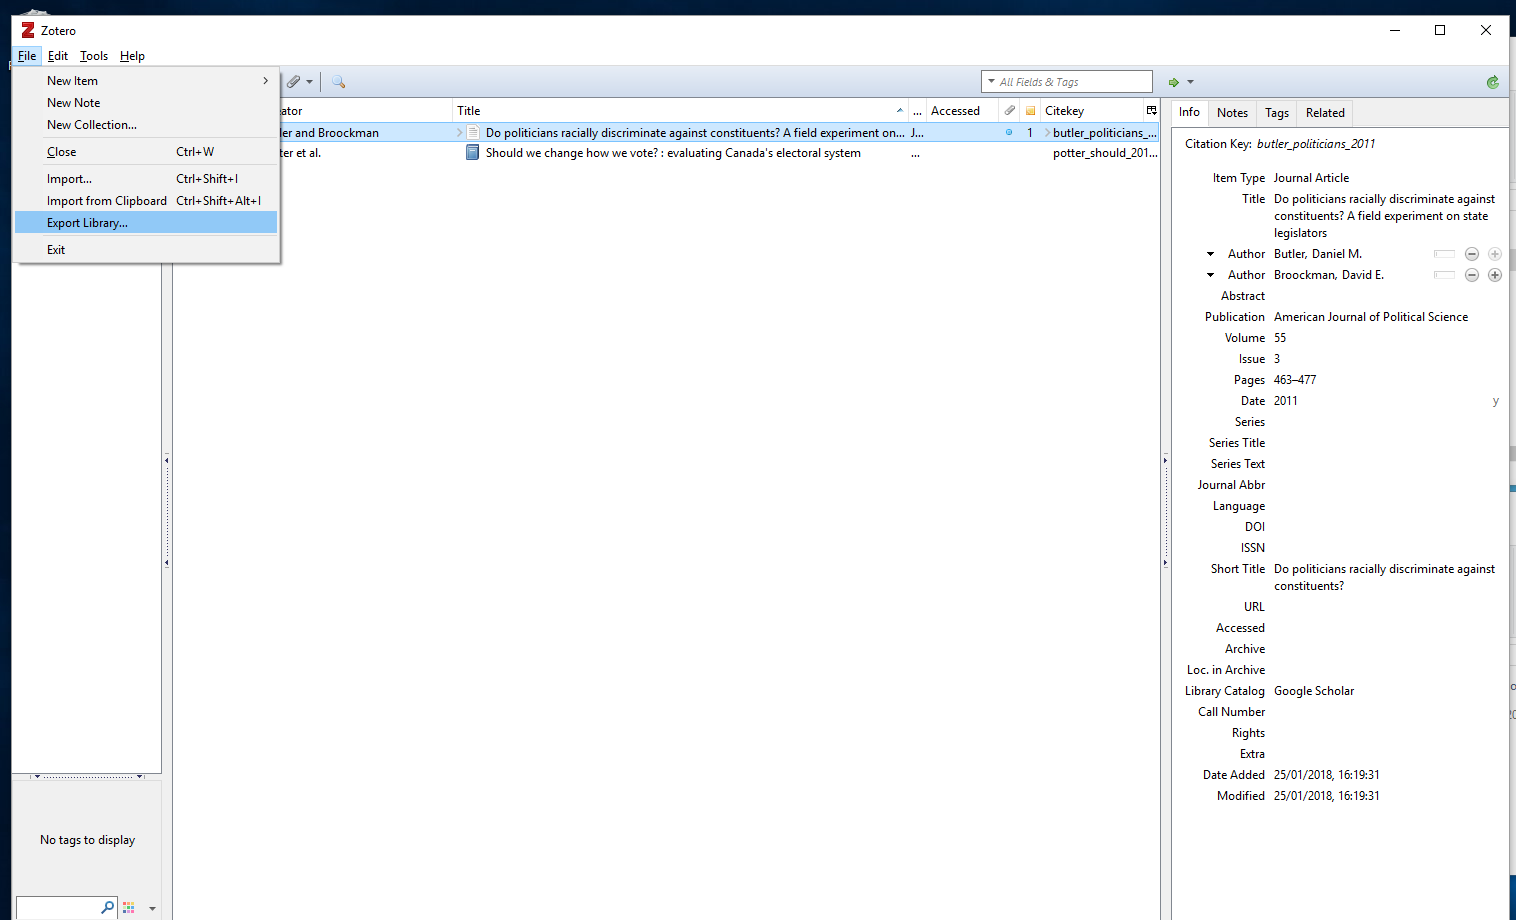
\includegraphics[height=3in, width = 4.25in,keepaspectratio]{zotero/bibtex_6.png}
\end{figure} \end{frame}

\begin{frame} \frametitle{Bib 7: We want a Better bibLaTeX} \begin{figure}[!h] \centering
	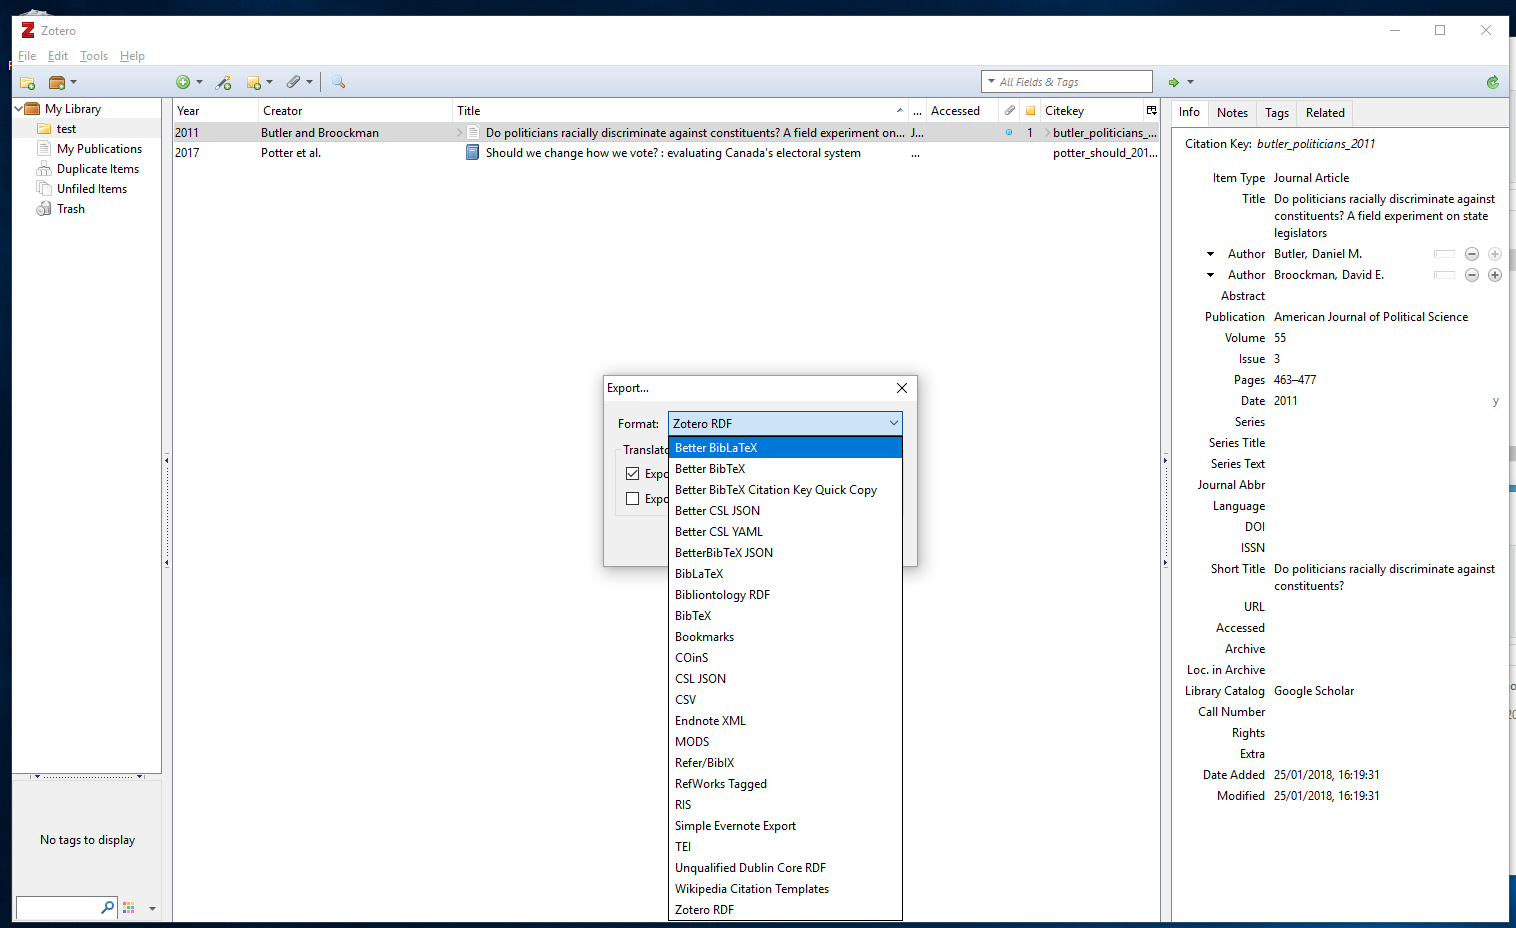
\includegraphics[height=3in, width = 4.25in,keepaspectratio]{zotero/bibtex_7.png}
\end{figure} \end{frame}

\begin{frame} \frametitle{Bib 8: Make sure to keep it updated} \begin{figure}[!h] \centering
	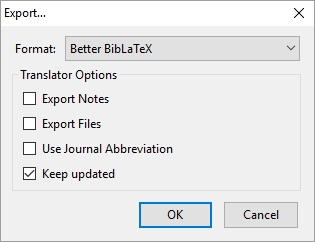
\includegraphics[height=3in, width = 4.25in,keepaspectratio]{zotero/bibtex_8.png}
\end{figure} \end{frame}

\begin{frame} \frametitle{Bib 9: Et voila! Try adding a citation} \begin{figure}[!h] \centering
	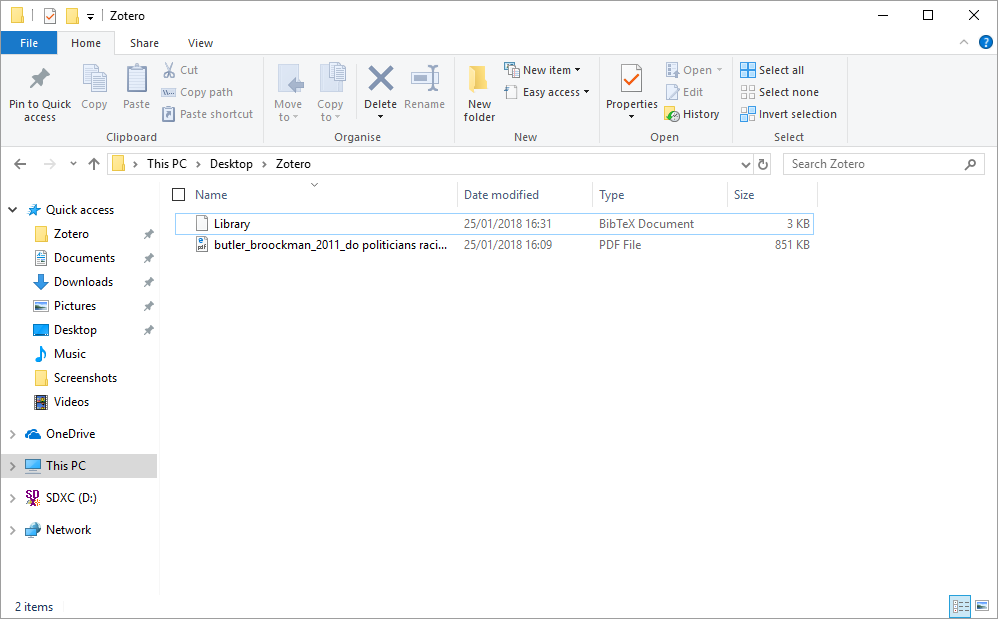
\includegraphics[height=3in, width = 4.25in,keepaspectratio]{zotero/bibtex_9.png}
\end{figure} \end{frame}

\end{document}